\section{Istruzioni all'uso}
% \subsection{Login}
\subsection{Home}
All'avvio del prodotto viene presentata la pagina \textit{Home}, da cui si può accedere alla barra di ricerca e degli strumenti, alle varie \href{https://7last.github.io/docs/pb/documentazione-interna/glossario\#dashboard}{\textit{dashboard}\textsubscript{G}} disponibili e al menù a tendina presente in angolo a sinistra.
\begin{center}
    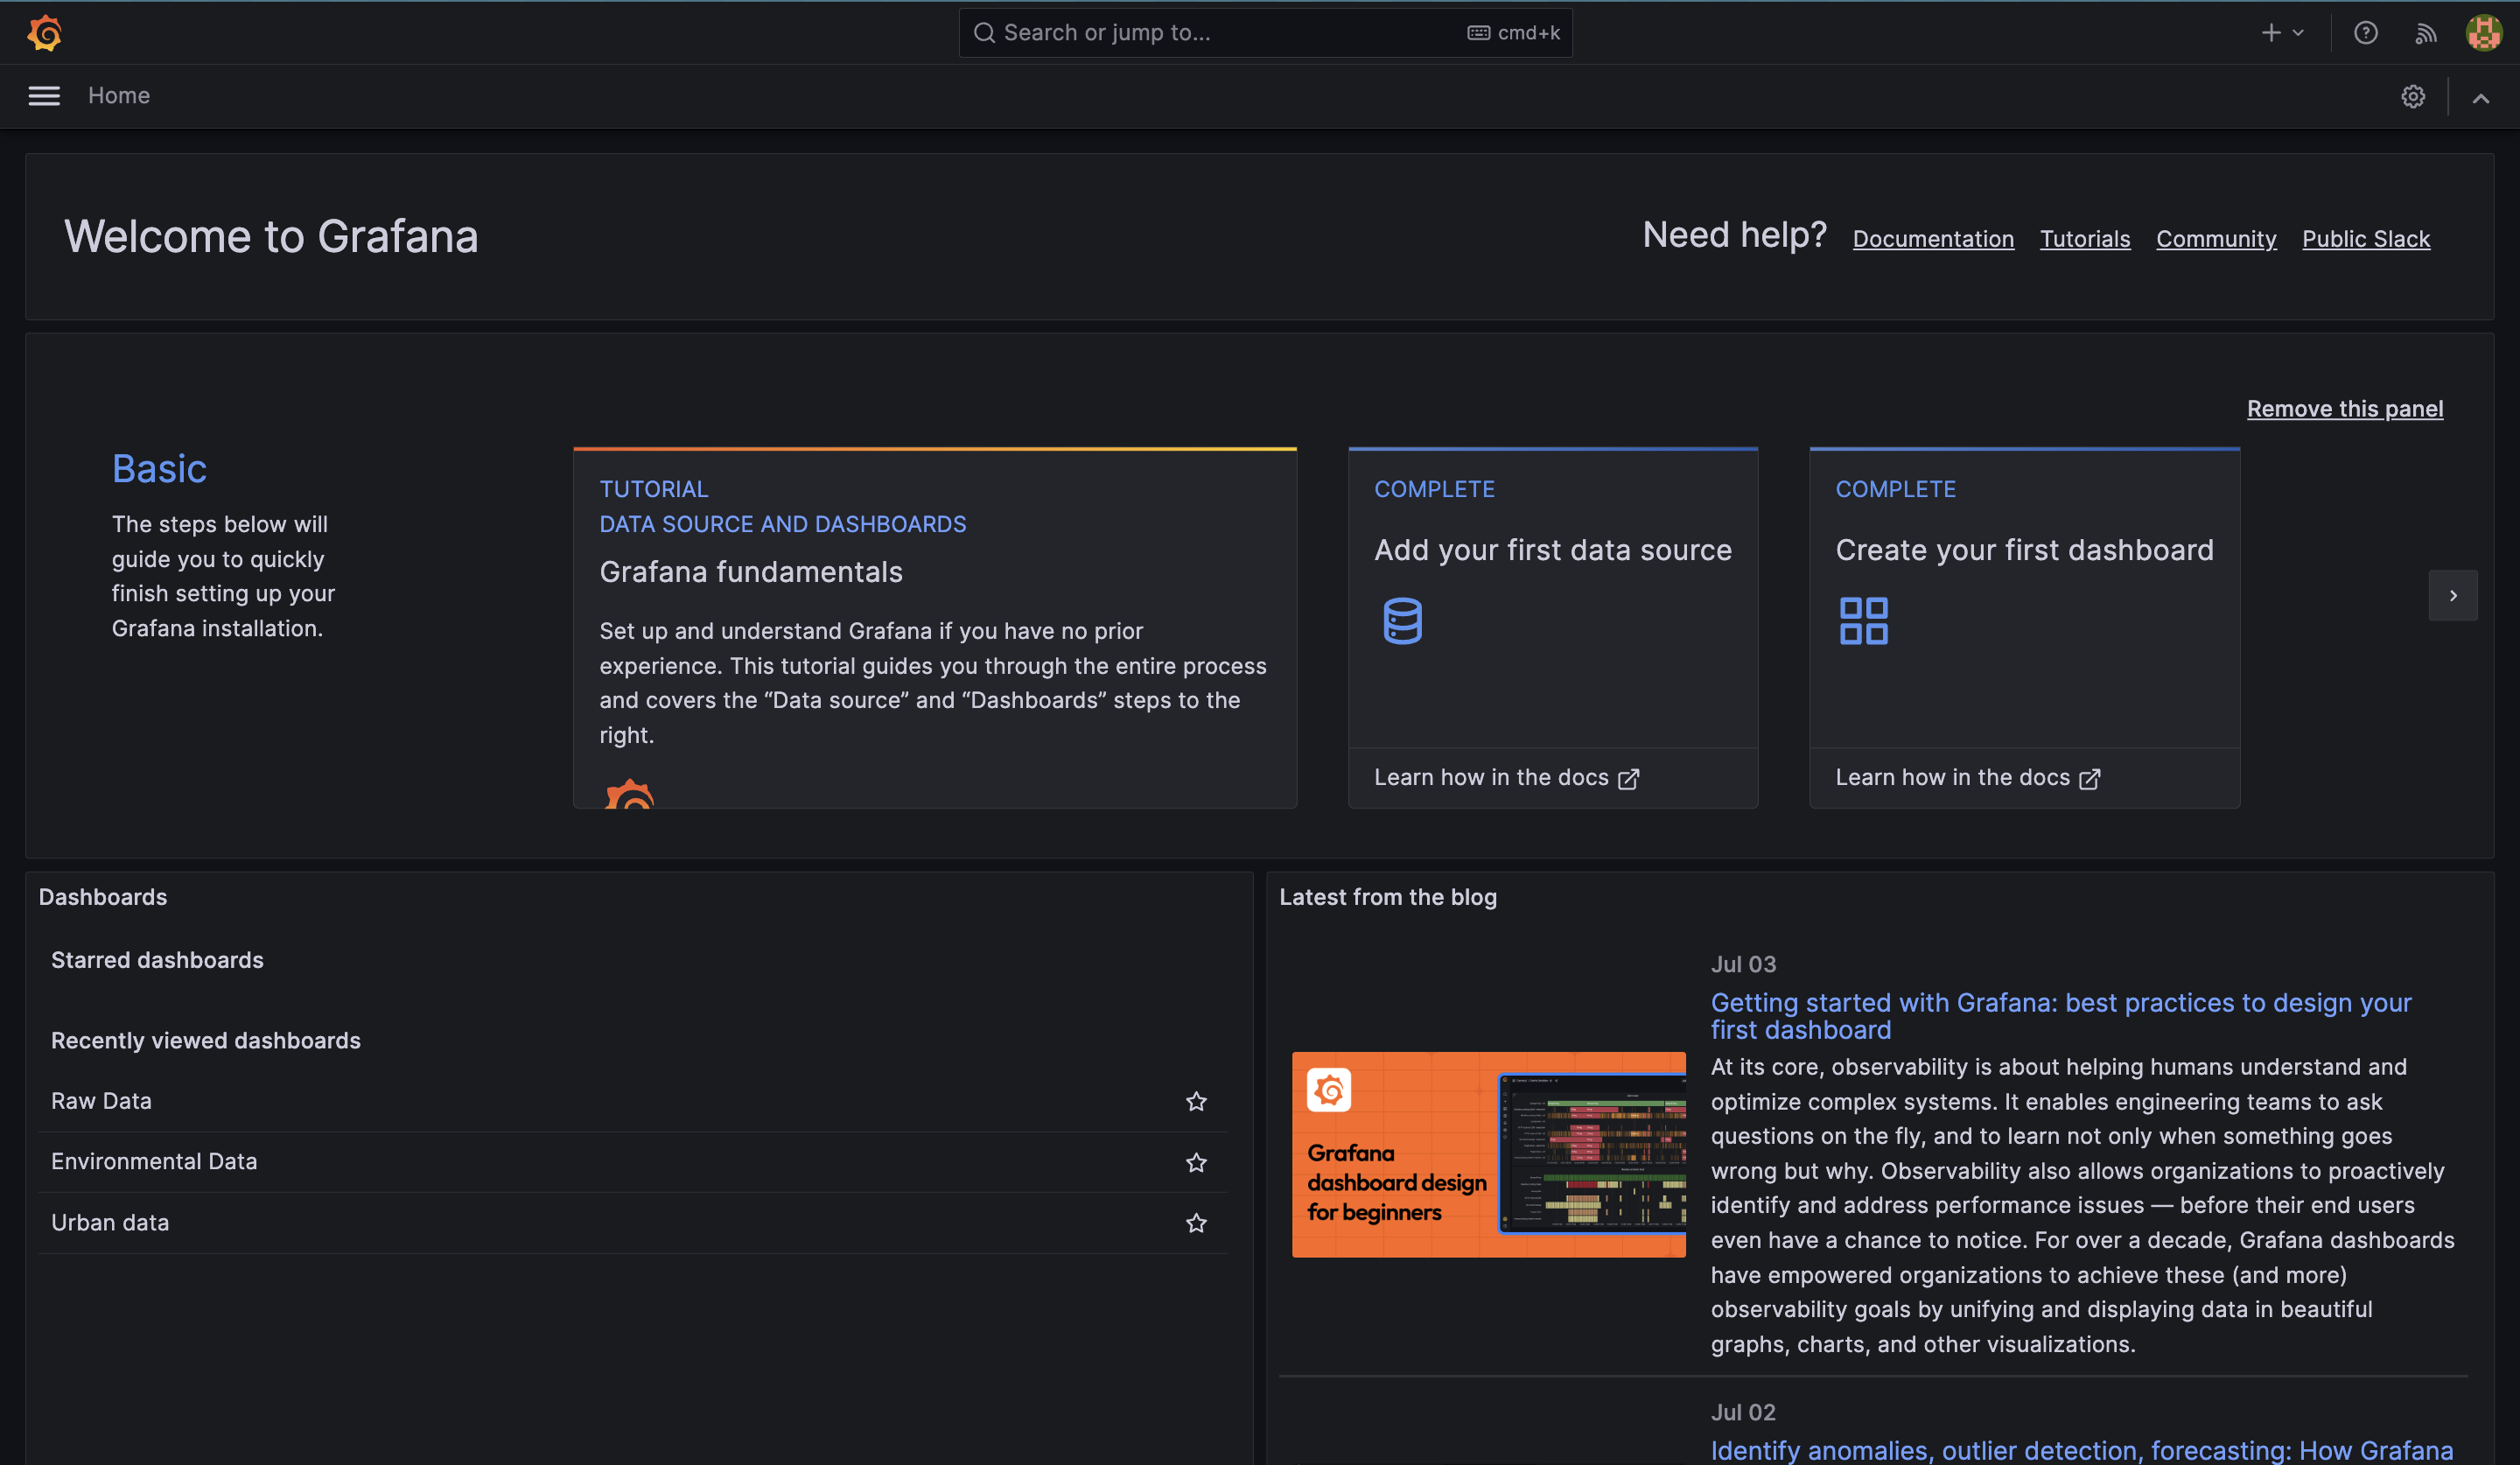
\includegraphics[width=\textwidth]{manuale_utente/General/home.png}
    \captionof{figure}{Schermata di accesso}
\end{center}
\newpage
\subsubsection{Barra di ricerca}
Permette un filtraggio rapido e preciso delle varie pagine presenti nell'applicazione. 
\begin{center}
    
\includegraphics[width=\textwidth]{manuale_utente/General/barra_ricerca.png}
    \captionof{figure}{Barra di ricerca}
\end{center}

\subsubsection{Barra degli strumenti}
Progettata per fornire all'utente un accesso immediato a una serie di funzionalità e azioni utili. Qui si possono trovare opzioni per personalizzare la visualizzazione dei dati, eseguire interrogazioni avanzate, gestire allarmi e condividere i risultati.
\begin{center}
    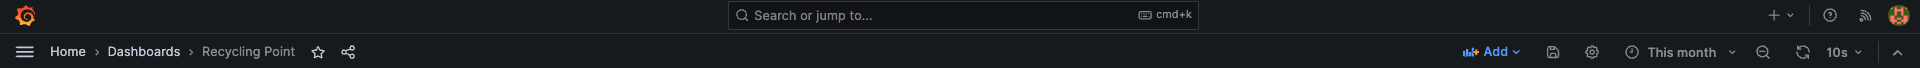
\includegraphics[width=\textwidth]{manuale_utente/General/barra_strumenti.png}
    \captionof{figure}{Barra degli strumenti}
\end{center}
Al suo interno vi sono ulteriori funzionalità, pensate per facilitare l'interazione con l'applicazione. In ordine da sinistra verso destra troviamo:
\begin{itemize}
    \item \textbf{menù a tendina}, che permette di accedere ad alcune sezioni fondamentali per lo scopo ultimo, tra cui:
        \begin{itemize}
            \item \textbf{\textit{Starred}}, in cui sono presenti le \href{https://7last.github.io/docs/pb/documentazione-interna/glossario\#dashboard}{\textit{dashboard}\textsubscript{G}} preferite;
            \item \textbf{\textit{Dashboards}}, dove è possibile vedere le \href{https://7last.github.io/docs/pb/documentazione-interna/glossario\#dashboard}{\textit{dashboard}\textsubscript{G}} disponibili;
            \item \textbf{\textit{Alerting}}, contenente tutte le notifiche e gli allarmi attivi.
        \end{itemize}
        \begin{center}
            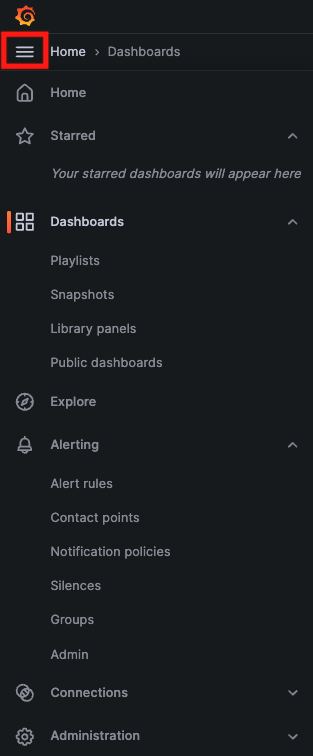
\includegraphics[width=0.2\textwidth]{manuale_utente/General/menu_tendina.png}
            \captionof{figure}{Menù a tendina}
        \end{center}
    \item \textbf{Breadcrumb}, mostra la posizione attuale dell'utente all'interno dell'applicazione.
        \begin{center}
            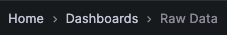
\includegraphics[width=0.9\textwidth]{manuale_utente/General/breadcrumb.png}
            \captionof{figure}{Breadcrumb}
        \end{center}
    \item \textbf{Favorite mark}, permette di aggiungere o rimuovere una \href{https://7last.github.io/docs/pb/documentazione-interna/glossario\#dashboard}{\textit{dashboard}\textsubscript{G}} dall'elenco preferiti.
        \begin{center}
            
\includegraphics[width=0.9\textwidth]{manuale_utente/General/favourite_mark.png}
            \captionof{figure}{Favorite mark}
        \end{center}
    \item \textbf{Share \href{https://7last.github.io/docs/pb/documentazione-interna/glossario\#dashboard}{dashboard\textsubscript{G}}}, consente di condividere la \href{https://7last.github.io/docs/pb/documentazione-interna/glossario\#dashboard}{\textit{dashboard}\textsubscript{G}} in questione.
        \begin{center}
            
\includegraphics[width=0.9\textwidth]{manuale_utente/General/share.png}
            \captionof{figure}{Share \href{https://7last.github.io/docs/pb/documentazione-interna/glossario\#dashboard}{dashboard\textsubscript{G}}}
        \end{center}
    \item \textbf{Add button}, permette di aggiungere un nuovo pannello alla \href{https://7last.github.io/docs/pb/documentazione-interna/glossario\#dashboard}{\textit{dashboard}\textsubscript{G}} selezionata.
        \begin{center}
            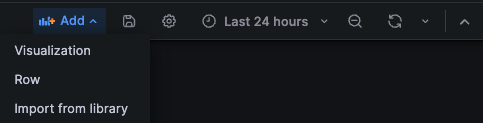
\includegraphics[width=0.9\textwidth]{manuale_utente/General/add_button.png}
            \captionof{figure}{Add button}
        \end{center}
    \item \textbf{Save \href{https://7last.github.io/docs/pb/documentazione-interna/glossario\#dashboard}{dashboard\textsubscript{G}}}, consente di salvare le modifiche apportate.
        \begin{center}
            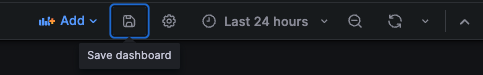
\includegraphics[width=0.9\textwidth]{manuale_utente/General/save.png}
            \captionof{figure}{Save \href{https://7last.github.io/docs/pb/documentazione-interna/glossario\#dashboard}{dashboard\textsubscript{G}}}
        \end{center}
    \newpage
    \item \href{https://7last.github.io/docs/pb/documentazione-interna/glossario\#dashboard}{\textbf{Dashboard}\textsubscript{G}}\textbf{ settings}, permette una personalizzazione della \href{https://7last.github.io/docs/pb/documentazione-interna/glossario\#dashboard}{\textit{dashboard}\textsubscript{G}} attuale.
        \begin{center}
            
\includegraphics[width=0.9\textwidth]{manuale_utente/General/settings.png}
            \captionof{figure}{\href{https://7last.github.io/docs/pb/documentazione-interna/glossario\#dashboard}{Dashboard\textsubscript{G}} settings}
        \end{center}
    \item \textbf{Time range}, consente di selezionare l'intervallo temporale dei dati visualizzati.
        \begin{center}
            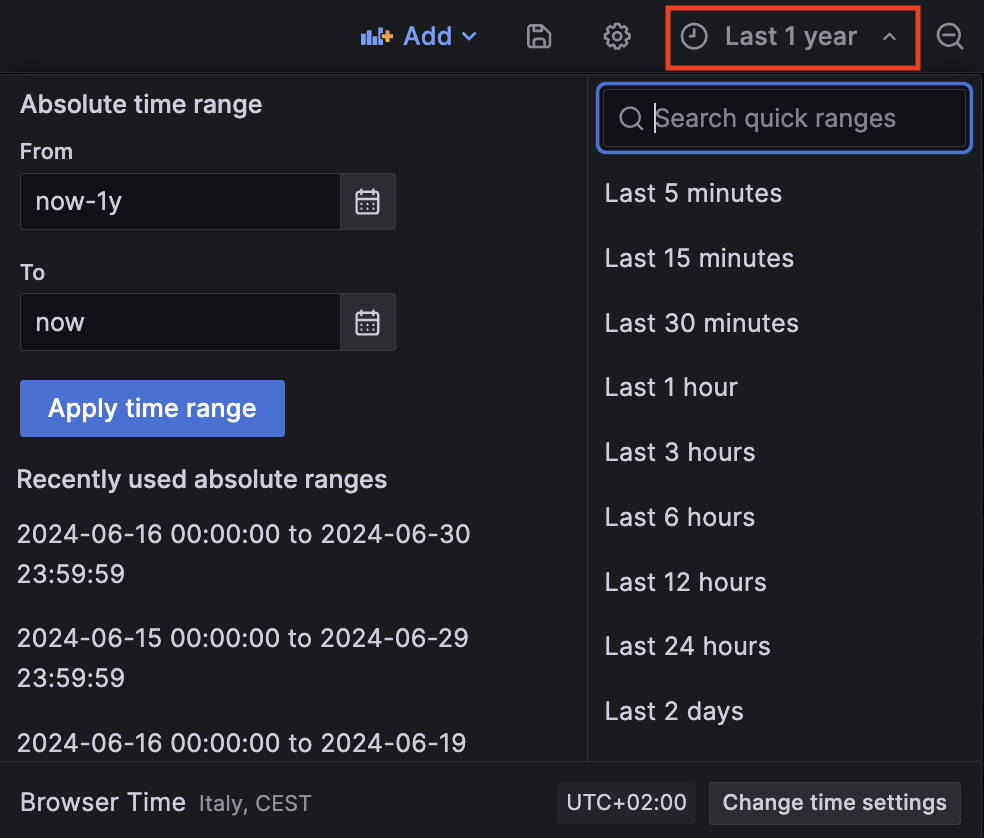
\includegraphics[width=0.5\textwidth]{manuale_utente/General/time_range.png}
            \captionof{figure}{Time range}
        \end{center}
    \item \textbf{Refresh}, permette di aggiornare i dati visualizzati oppure impostare una frequenza di aggiornamento automatico.
        \begin{center}
            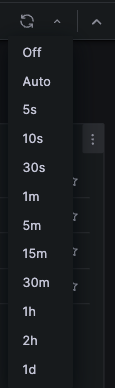
\includegraphics[width=0.06\textwidth]{manuale_utente/General/refresh.png}
            \captionof{figure}{Refresh}
        \end{center}
\end{itemize}

\subsection{Dashboard}
Costituiscono il cuore pulsante dell'applicazione e sono progettate per fornire una visualizzazione intuitiva e dettagliata dei dati raccolti dai sensori. Ogni \href{https://7last.github.io/docs/pb/documentazione-interna/glossario\#dashboard}{\textit{dashboard}\textsubscript{G}} è suddivisa in righe dedicate, ciascuna contenente dei pannelli focalizzati su un aspetto specifico dell'analisi o del monitoraggio.

\subsubsection{Pannelli}
Ogni pannello racchiude dati pertinenti rappresentati attraverso grafici e altre visualizzazioni e offre una panoramica chiara e dettagliata su un determinato aspetto dell'analisi o del monitoraggio. Ciascun pannello contiene:
\begin{itemize}
    \item titolo;
    \item informazioni in merito al \href{https://7last.github.io/docs/pb/documentazione-interna/glossario\#sensore}{sensore\textsubscript{G}};
    \item menù a tendina (se presente);
    \item legenda (se presente);
    \item visualizzazione dei dati misurati.
\end{itemize}

\subsubsection{Tipologie di grafici}
\subsubsubsection*{Mappa}
Visualizza la posizione dei sensori su una mappa interattiva. Mediante i pulsanti "+" e "-" vi è la possibilità di ingrandire o ridurre la mappa, consentendo di vedere più dettagli o una vista più ampia. Cliccando su un marker del \href{https://7last.github.io/docs/pb/documentazione-interna/glossario\#sensore}{sensore\textsubscript{G}}, si aprirà un popup con informazioni dettagliate sul \href{https://7last.github.io/docs/pb/documentazione-interna/glossario\#sensore}{sensore\textsubscript{G}} corrispondente. È inoltre possibile spostarsi sulla mappa trascinando il mouse per una navigazione fluida all'interno dell'area rappresentata. Nell'angolo in basso a sinistra è disponibile una legenda che identifica i diversi tipi di sensori presenti sulla mappa.
\begin{center}
    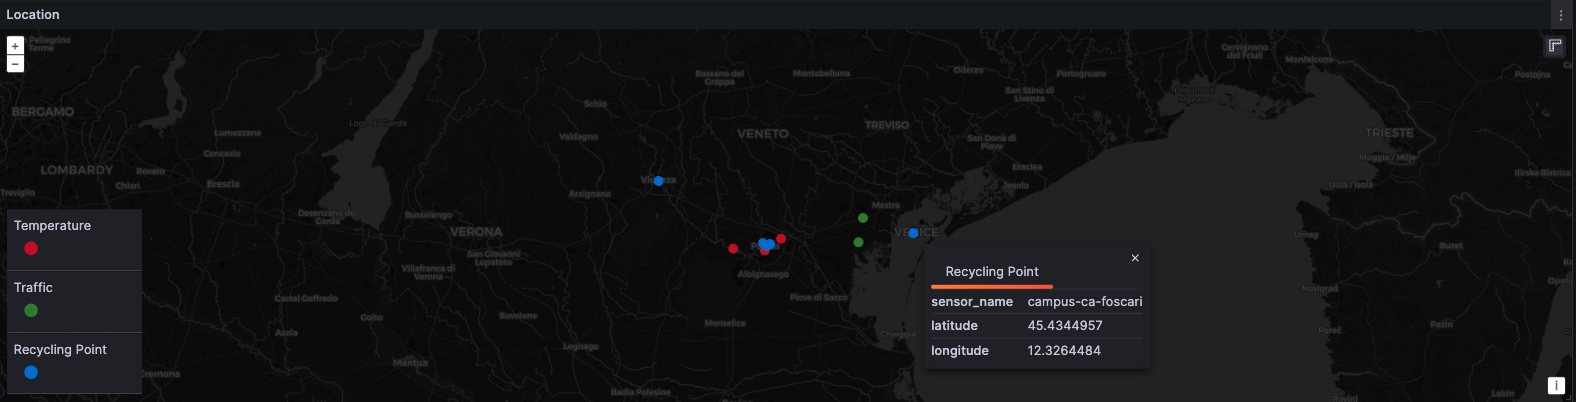
\includegraphics[width=\textwidth]{manuale_utente/General/mappa.png}
    \captionof{figure}{Mappa dei sensori}
\end{center}

\subsubsubsection*{Grafico a linee} 
Rappresenta i dati tramite linee, con l'asse x che indica il tempo e l'asse y il valore misurato. È possibile mostrare più serie di dati simultaneamente, facilitando il confronto tra dati provenienti da diversi sensori o categorie.
\begin{center}
    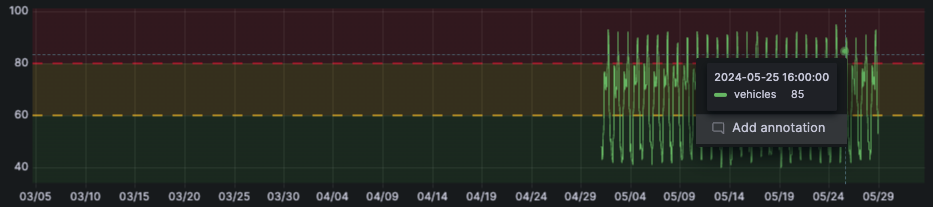
\includegraphics[width=\textwidth]{manuale_utente/General/time_series.png}
    \captionof{figure}{Grafico a linee}
\end{center} 
\newpage

% \subsubsubsection*{Statistiche}
% Fornisce un'istantanea del valore misurato, mostrando ad esempio un numero o un indicatore visivo come una freccia o un'icona. Utile per monitorare un singolo dato in tempo reale e per evidenziare eventuali anomalie o variazioni significative.
% \begin{center}
%     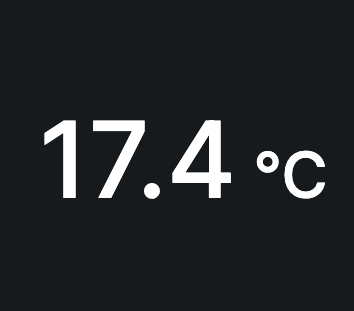
\includegraphics[width=0.4\textwidth]{manuale_utente/General/stat.png}
%     \captionof{figure}{Grafico per le statistiche}
% \end{center} 

\subsubsubsection*{Grafico a quadrante}
Divide i dati in tre quadranti, ciascuno rappresentato da un colore diverso. Ogni quadrante corrisponde a un intervallo di valori specifico, consentendo di identificare rapidamente se il valore misurato è inferiore, superiore o all'interno di un determinato intervallo. È particolarmente utile per valutare le prestazioni rispetto a obiettivi o soglie prestabilite.
\begin{center}
    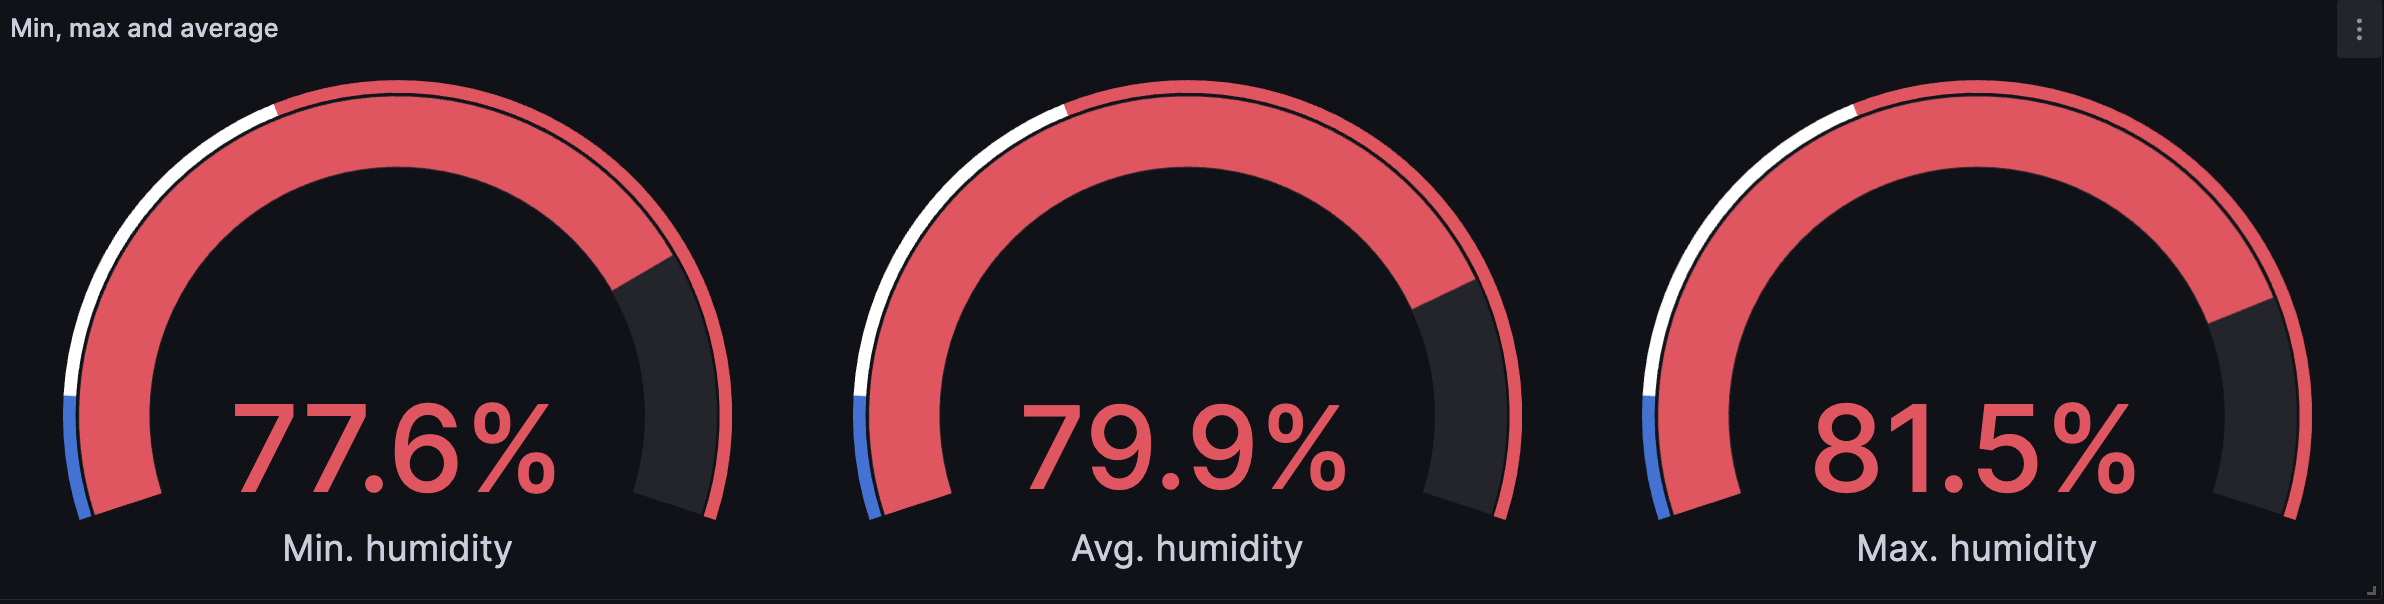
\includegraphics[width=\textwidth]{manuale_utente/General/grafico_quadrante.png}
    \captionof{figure}{Grafico a quadrante}
\end{center}

\subsubsubsection*{Grafico a barre}
Visualizza i dati in forma di barre orizzontali o verticali, con l'altezza o la lunghezza della barra proporzionale al valore misurato. 
\begin{center}
    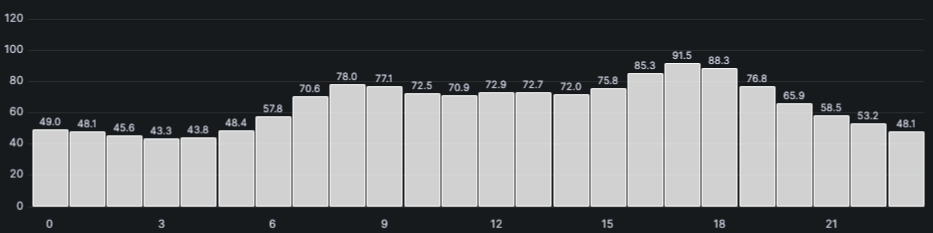
\includegraphics[width=0.8\textwidth]{manuale_utente/General/grafico_barre.png}
    \captionof{figure}{Grafico a barre}
\end{center}

\subsubsubsection*{Tabella}
Rappresenta i dati provenienti dai sensori in forma tabellare. Ogni riga della tabella corrisponde a un \href{https://7last.github.io/docs/pb/documentazione-interna/glossario\#sensore}{sensore\textsubscript{G}} e mostra le relative informazioni. Le colonne della tabella rappresentano le diverse categorie di dati, come valori misurati e timestamp della misurazione. La tabella fornisce una visione compatta e organizzata dei dati dei sensori, facilitando la ricerca e l'analisi delle informazioni.
\begin{center}
    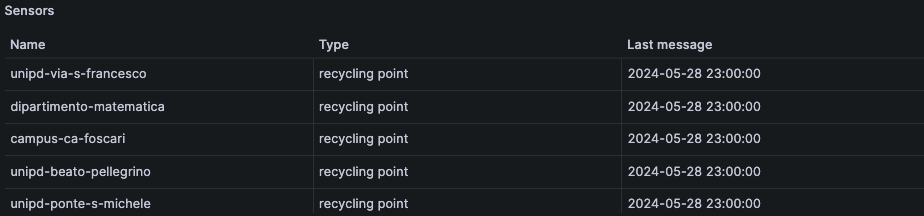
\includegraphics[width=\textwidth]{manuale_utente/General/tabelle.png}
    \captionof{figure}{Tabella}
\end{center} 


\subsubsection{Gestione sensori visualizzabili}
Abbiamo configurato dei filtri che permettono all'utente di visualizzare solo i sensori di interesse, selezionabili in base alla tipologia e/o al nome. Questo strumento è particolarmente utile quando si lavora con un gran numero di sensori e si desidera concentrarsi esclusivamente su quelli rilevanti per l'analisi o il monitoraggio corrente.
% \begin{center}
%     \includegraphics[width=\textwidth]{manuale_utente/.png}
%     \captionof{figure}{Filtri sensori}
% \end{center} 
\newpage
\subsection{Gruppi di pannelli}
\subsubsection{Raw Data}
La \href{https://7last.github.io/docs/pb/documentazione-interna/glossario\#dashboard}{\textit{dashboard}\textsubscript{G}} generale è suddivisa in righe, ciascuna delle quali contiene informazioni relative a specifiche tipologie di sensori. Permette di visualizzare la posizione dei sensori su una mappa interattiva, utilizzando una codifica a colori per differenziare le varie tipologie di sensori, come quelli per la temperatura, il traffico e le isole ecologiche. Inoltre include tabelle dettagliate con informazioni aggiornate per una comprensione immediata. La \href{https://7last.github.io/docs/pb/documentazione-interna/glossario\#dashboard}{\textit{dashboard}\textsubscript{G}} è organizzata dall'alto verso il basso e da sinistra verso destra nel seguente modo:
\begin{itemize}
    \item filtro per visualizzare i sensori di preferenza;
    \begin{center}
        
\includegraphics[width=0.7\textwidth]{manuale_utente/Rawdata/filtro_rawdata.png}
        \captionof{figure}{Filtro Raw Data}
    \end{center} 
    \item riga \textit{\textbf{Sensor}} contenente:
    \begin{itemize}
        \item mappa dei sensori;
        \begin{center}
            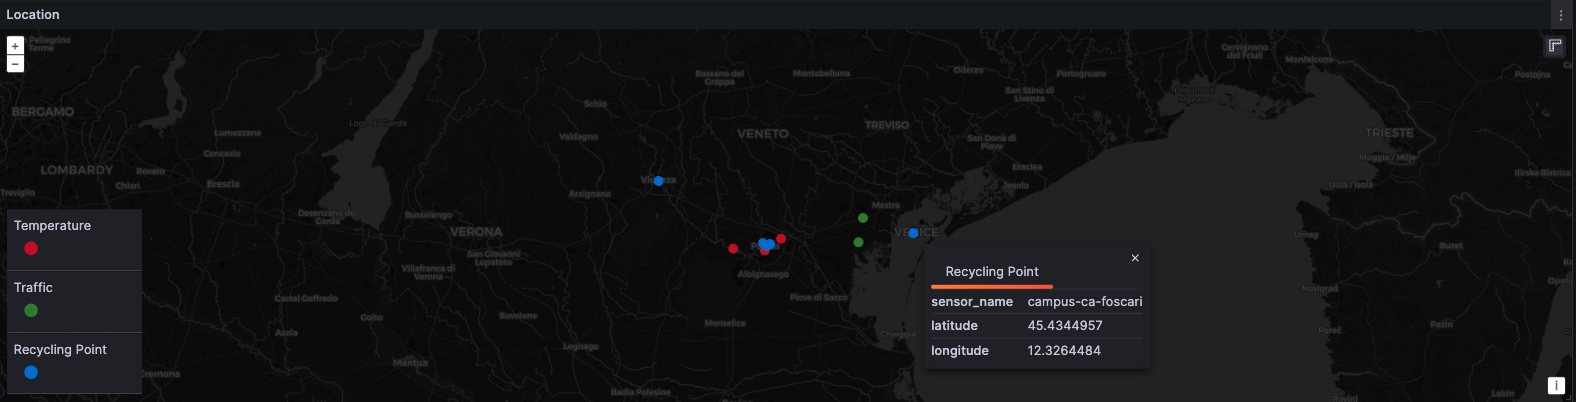
\includegraphics[width=0.7\textwidth]{manuale_utente/General/mappa.png}
            \captionof{figure}{Mappa sensori Raw Data}
        \end{center} 
        \item collegamento alle \href{https://7last.github.io/docs/pb/documentazione-interna/glossario\#dashboard}{\textit{dashboard}\textsubscript{G}} dettagliate;
        \begin{center}
            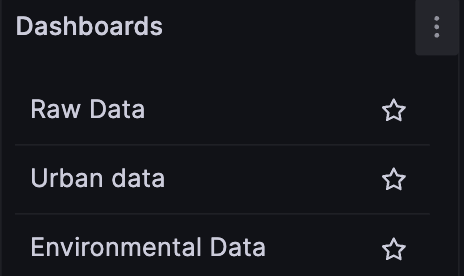
\includegraphics[width=0.7\textwidth]{manuale_utente/Rawdata/collegamento_rawdata.png}
            \captionof{figure}{Collegamento \href{https://7last.github.io/docs/pb/documentazione-interna/glossario\#dashboard}{\textit{dashboard}\textsubscript{G}} sensori Raw Data}
        \end{center} 
        \item tabella con tutti i sensori e l'ultima rilevazione effettuata;
        \begin{center}
            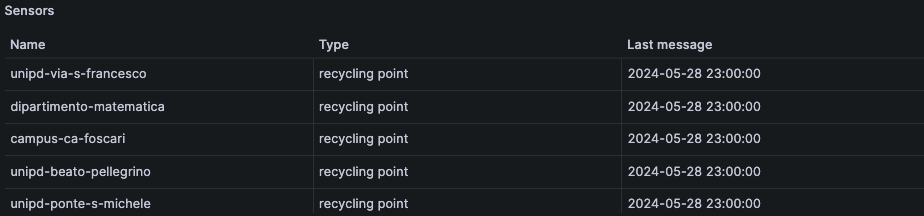
\includegraphics[width=0.7\textwidth]{manuale_utente/General/tabelle.png}
            \captionof{figure}{Tabella sensori Raw Data}
        \end{center} 
        \item grafico a barre orizzontali con il totale di sensori per tipo;
        \begin{center}
            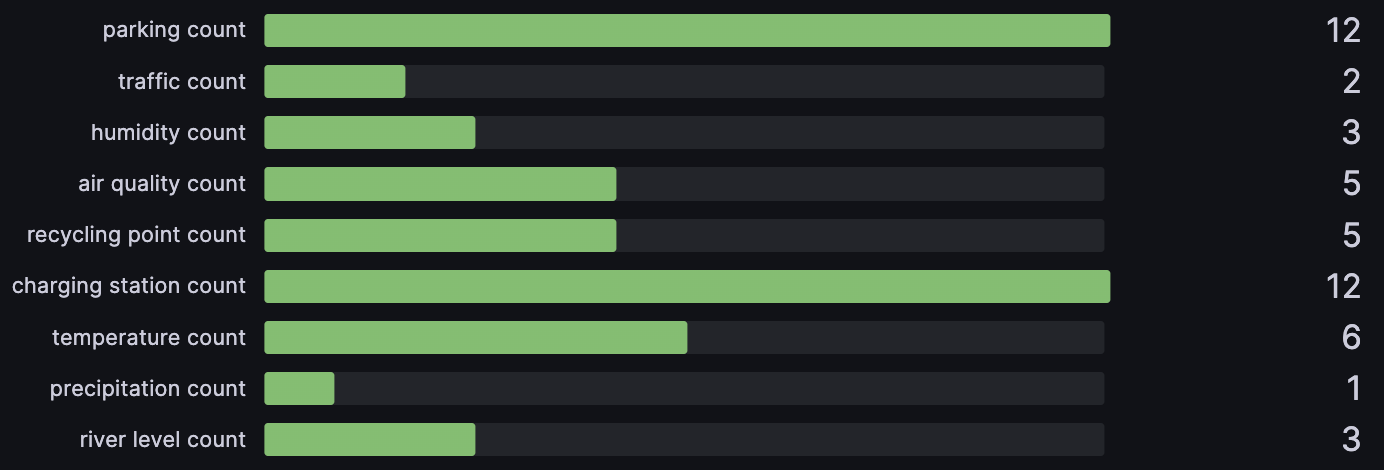
\includegraphics[width=0.7\textwidth]{manuale_utente/Rawdata/barre_rawdata.png}
            \captionof{figure}{Grafico conteggio sensori Raw Data}
        \end{center} 
    \end{itemize}
    \newpage
    \item riga \textit{\textbf{Air quality}} contenente:
    \begin{itemize}
        \item mappa della qualità dell'aria;
        \begin{center}
            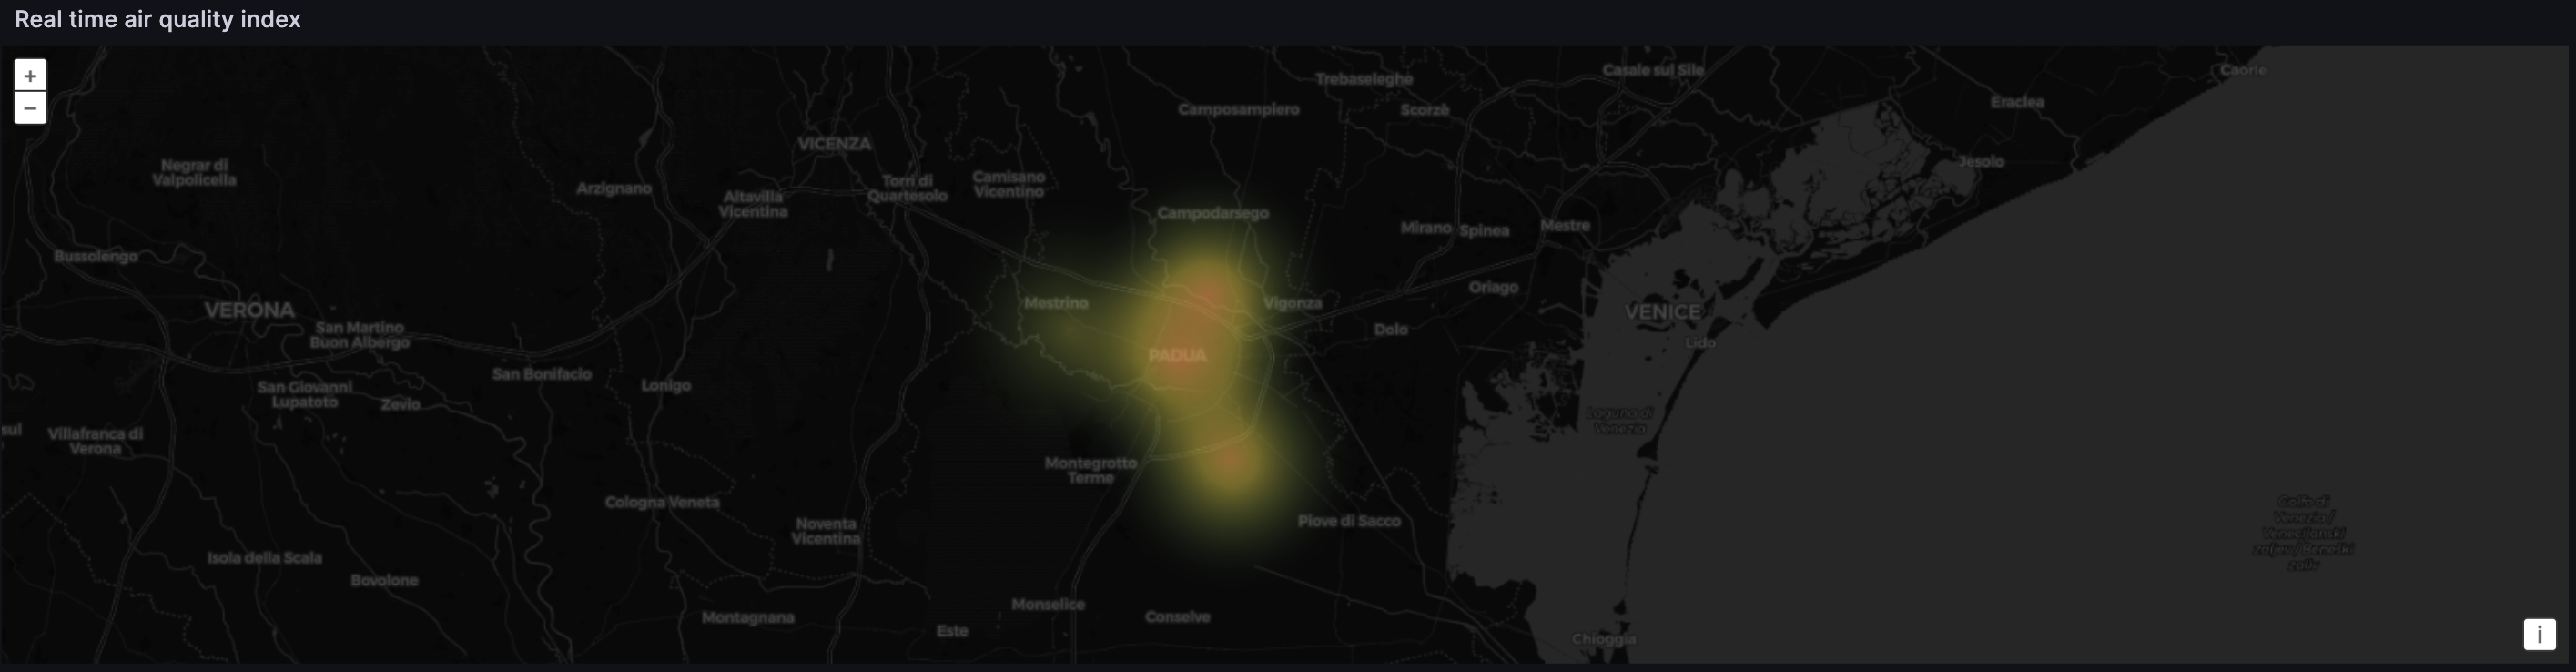
\includegraphics[width=0.7\textwidth]{manuale_utente/Rawdata/airquality_map.png}
            \captionof{figure}{Grafico qualità dell'aria Raw Data - Air quality}
        \end{center}
        \item tabella con gli ultimi dati raccolti;
        \begin{center}
            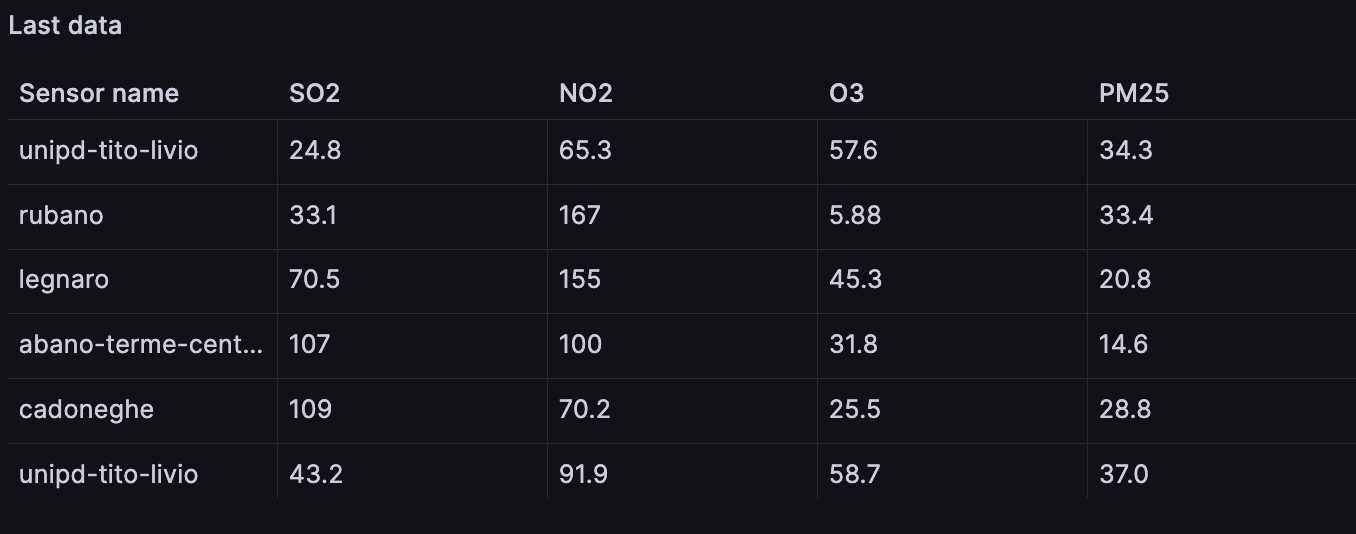
\includegraphics[width=0.7\textwidth]{manuale_utente/Rawdata/tabella_aria.png}
            \captionof{figure}{Tabella dati raccolti Raw Data - Air quality}
        \end{center}
        \item grafico a linee con lo storico dell'andamento degli agenti inquinanti;
        \begin{center}
            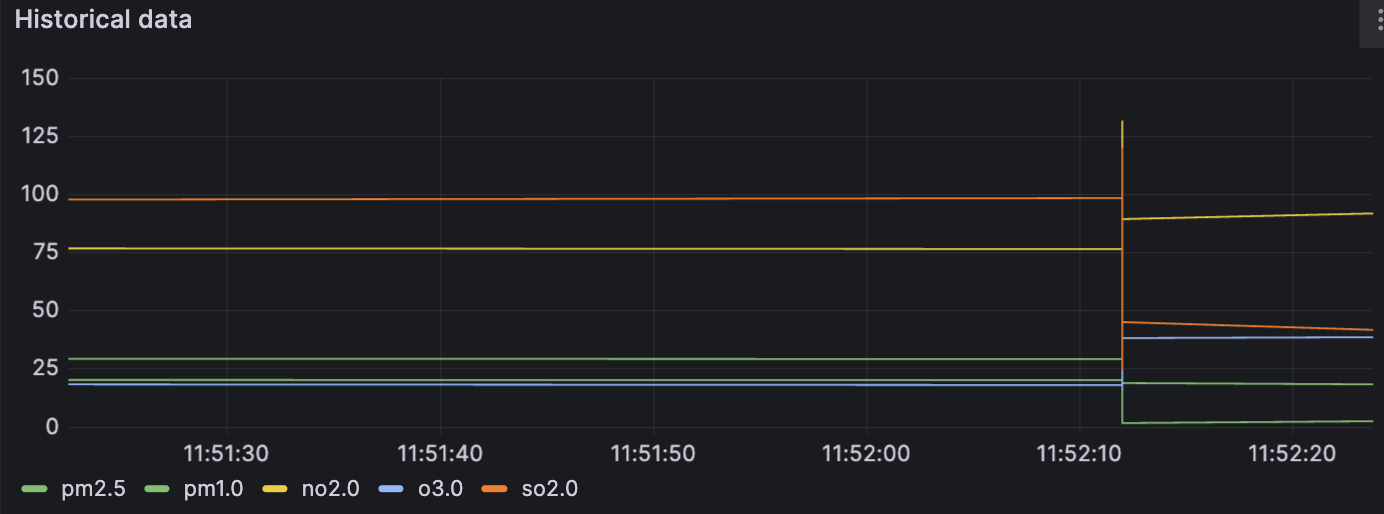
\includegraphics[width=0.7\textwidth]{manuale_utente/Rawdata/agenti_inquinanti.png}
            \captionof{figure}{Grafico agenti inquinanti Raw Data - Air quality}
        \end{center}
    \end{itemize}
    \item riga \textit{\textbf{Temperature}} contenente:
    \begin{itemize}
        \item tabella con gli ultimi dati raccolti;
        \begin{center}
            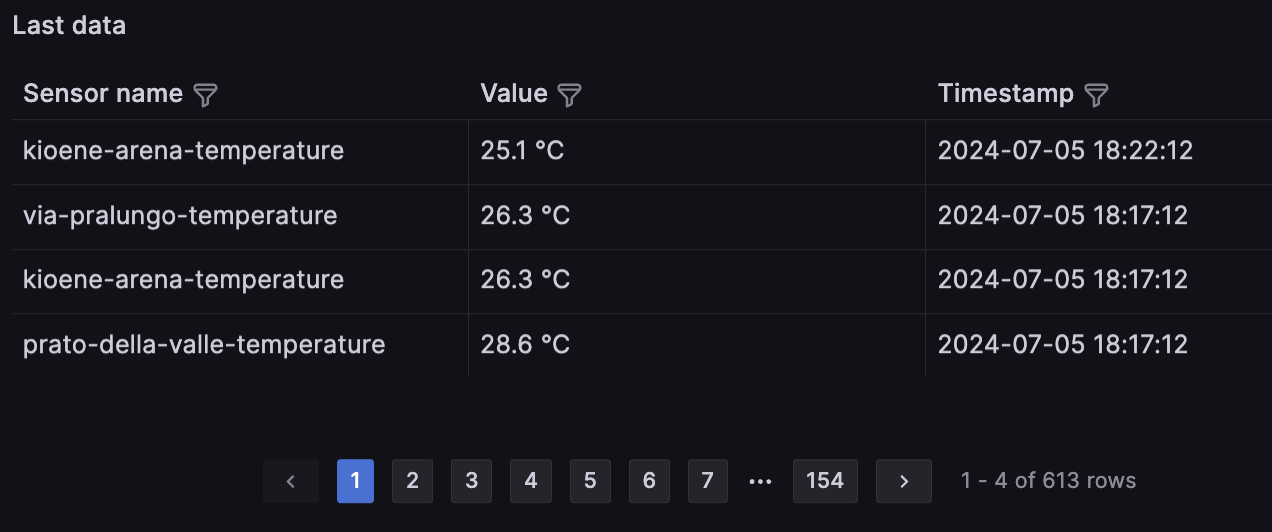
\includegraphics[width=0.7\textwidth]{manuale_utente/Rawdata/tabella_temperatura.png}
            \captionof{figure}{Tabella dati raccolti Raw Data - Temperature}
        \end{center}
        \item grafico a linee con lo storico dell'andamento della temperatura;
        \begin{center}
            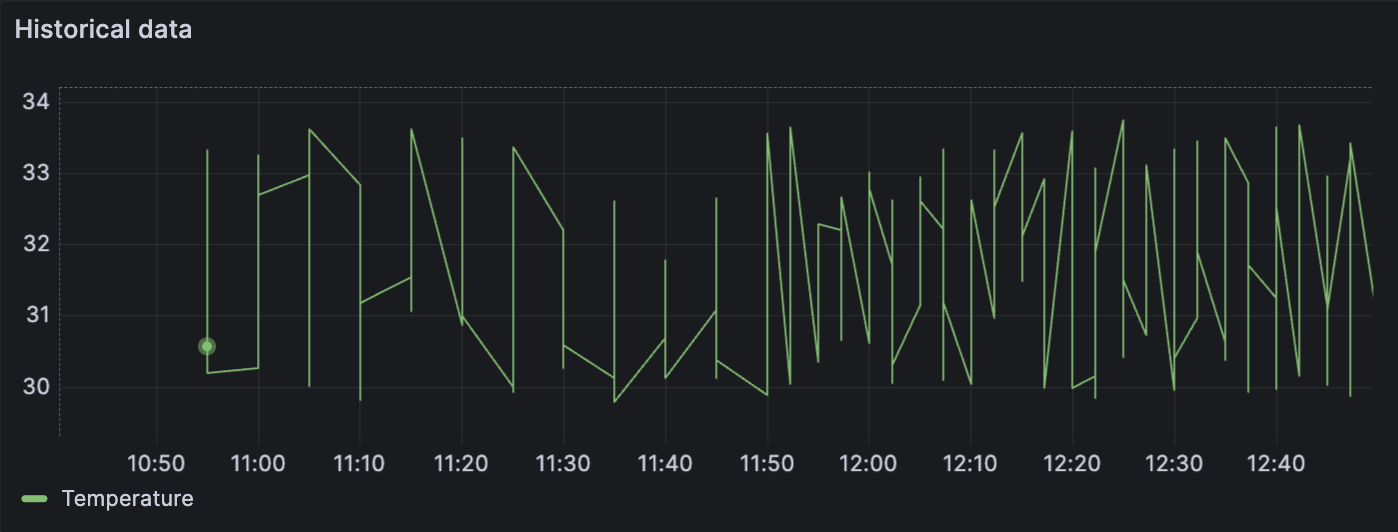
\includegraphics[width=0.7\textwidth]{manuale_utente/Rawdata/grafico_temperatura_rawdata.png}
            \captionof{figure}{Grafico Raw Data - Temperature}
        \end{center}
    \end{itemize}
    \item riga \textit{\textbf{Humidity}} contenente:
    \begin{itemize}
        \item tabella con gli ultimi dati raccolti;
        \begin{center}
            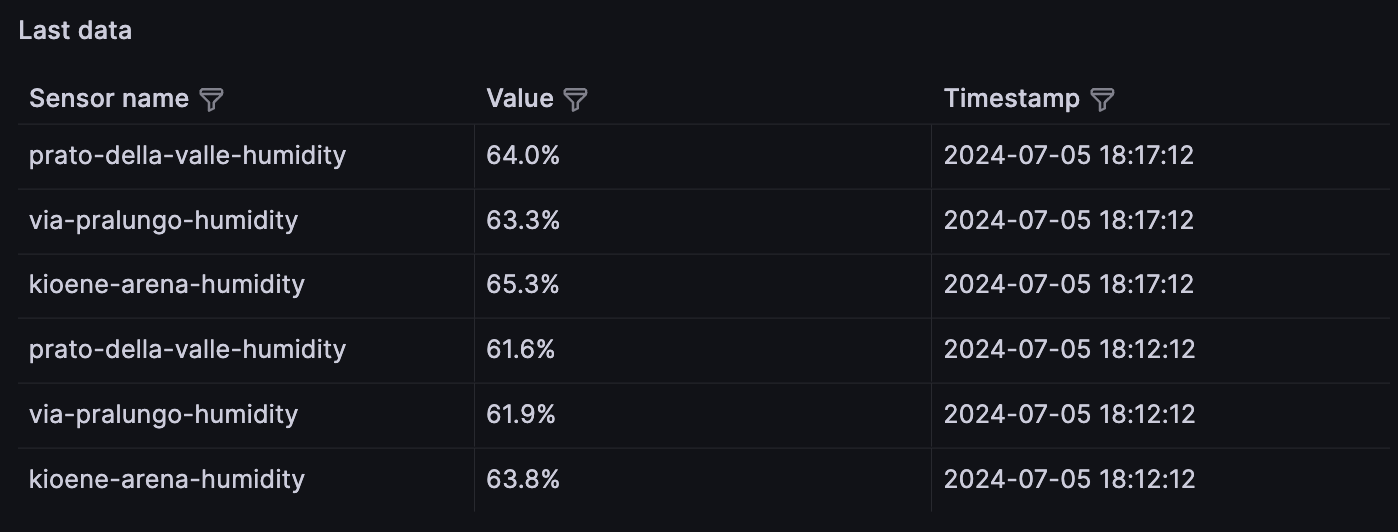
\includegraphics[width=0.7\textwidth]{manuale_utente/Rawdata/humidity_tables_rawdata.png}
            \captionof{figure}{Tabella dati raccolti Raw Data - Humidity}
        \end{center}
        \item grafico a linee con lo storico dell'andamento dell'umidità;
        \begin{center}
            \includegraphics[width=0.7\textwidth]{manuale_utente/Rawdata/grafico_umidità_rawdata.png}
            \captionof{figure}{Grafico Raw Data - Humidity}
        \end{center}
    \end{itemize}
    \item riga \textit{\textbf{Parking}} contenente:
    \begin{itemize}
        \item tabella con gli ultimi dati raccolti;
        \begin{center}
            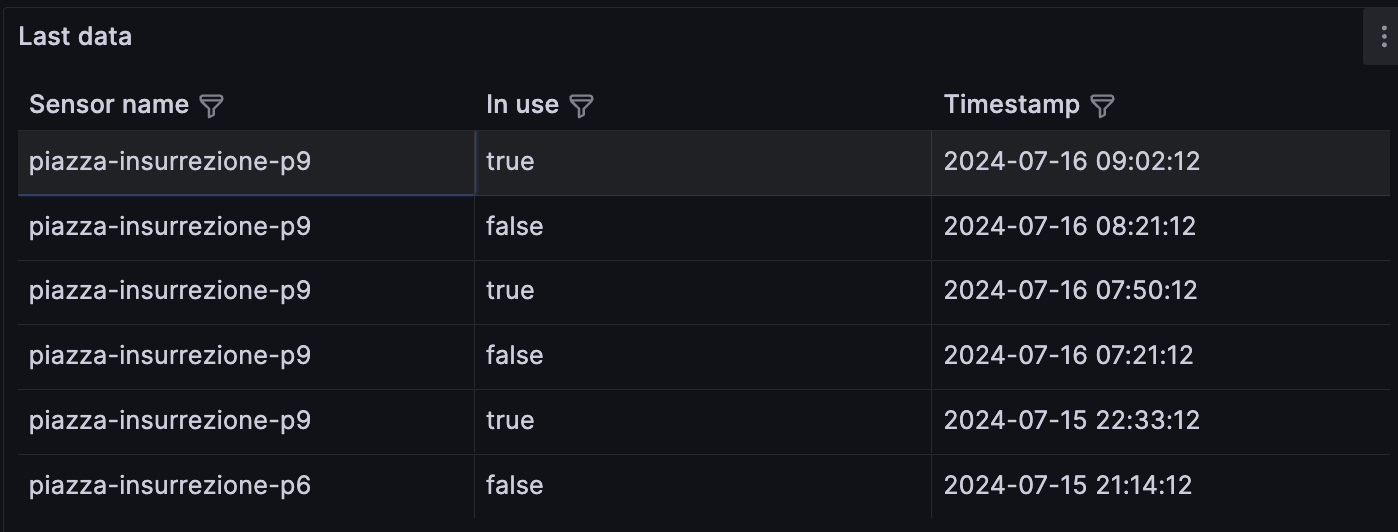
\includegraphics[width=0.7\textwidth]{manuale_utente/Rawdata/parking_table_rawdata.png}
            \captionof{figure}{Tabella dati raccolti Raw Data - Parking}
        \end{center}
        \item grafico a linee con lo storico dell'occupazione dei parcheggi;
        \begin{center}
            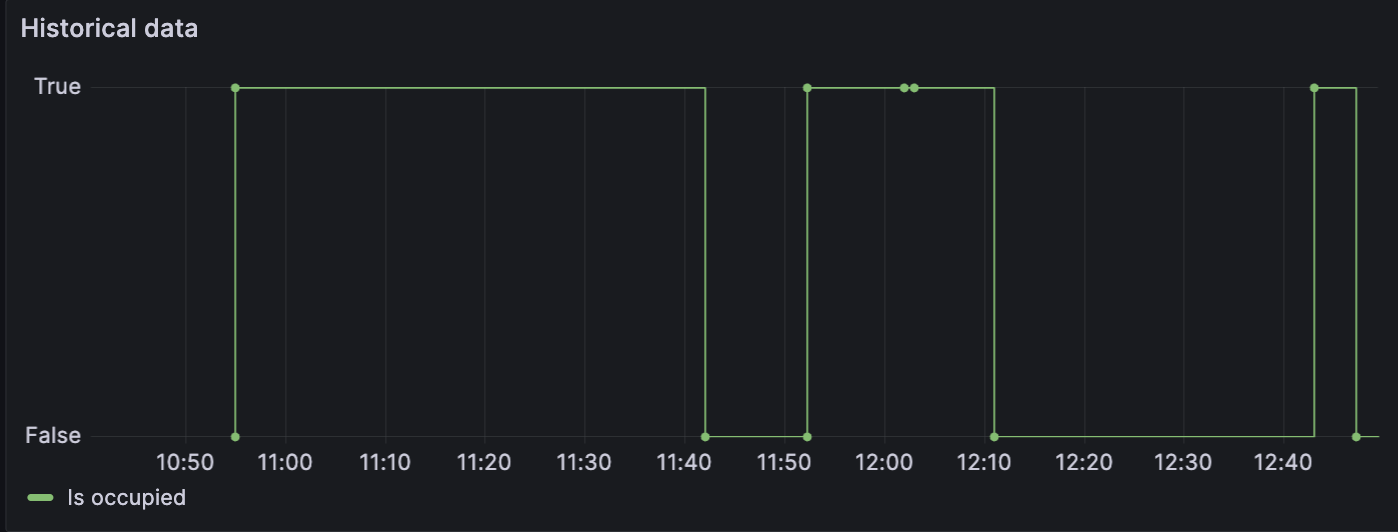
\includegraphics[width=0.7\textwidth]{manuale_utente/Rawdata/grafico_parking_rawdata.png}
            \captionof{figure}{Grafico occupazione Raw Data - Parking}
        \end{center}
    \end{itemize}
    \item riga \textit{\textbf{Charging}} contenente:
    \begin{itemize}
        \item tabella con gli ultimi dati raccolti;
        \begin{center}
            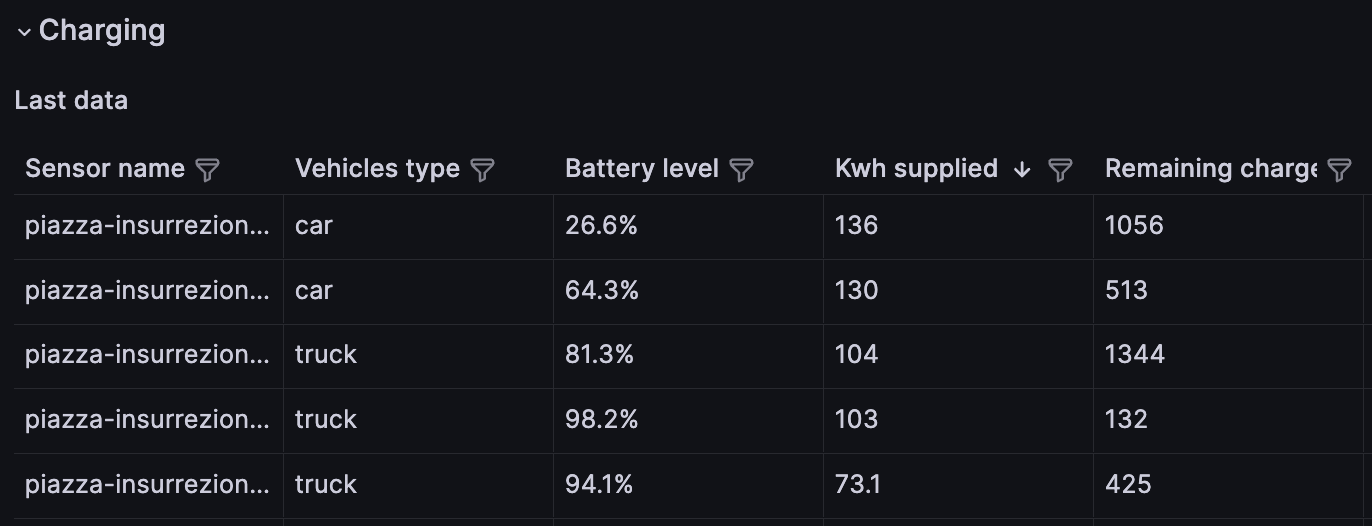
\includegraphics[width=0.7\textwidth]{manuale_utente/Rawdata/charging_table_rawdata.png}
            \captionof{figure}{Tabella dati raccolti Raw Data - Charging station}
        \end{center}
        \item grafico a linee con lo storico dell'occupazione delle colonnine di ricarica;
        \begin{center}
            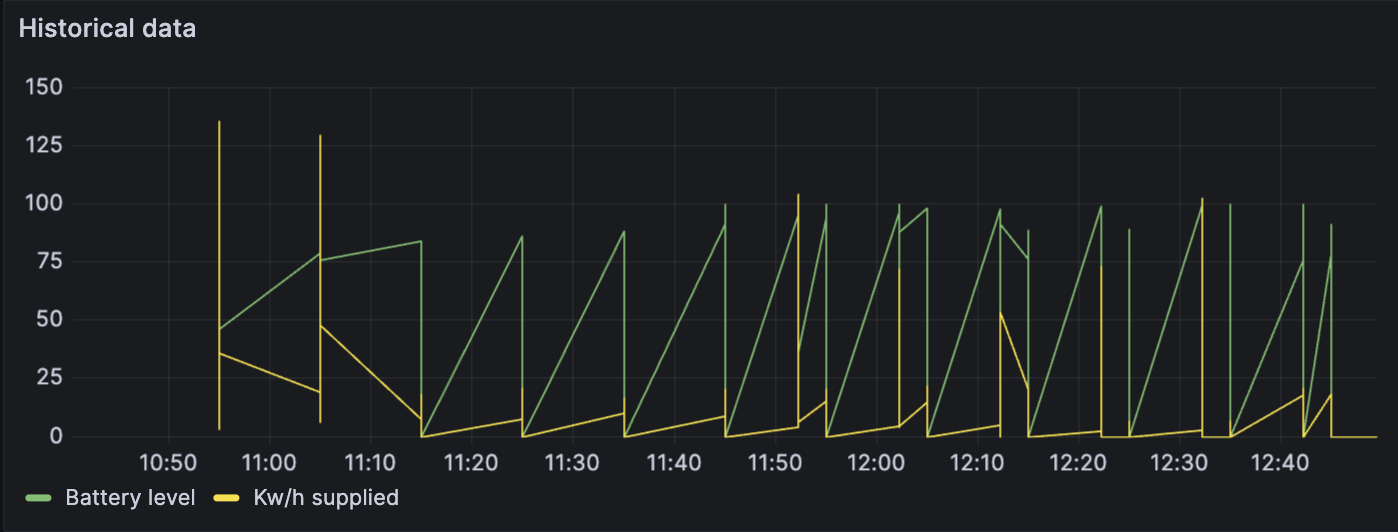
\includegraphics[width=0.7\textwidth]{manuale_utente/Rawdata/grafico_charging_rawdata.png}
            \captionof{figure}{Grafico occupazione colonnine ricarica Raw Data - Charging station}
        \end{center}
    \end{itemize}
    \item riga \textit{\textbf{Precipitation}} contenente:
    \begin{itemize}
        \item tabella con gli ultimi dati raccolti;
        \begin{center}
            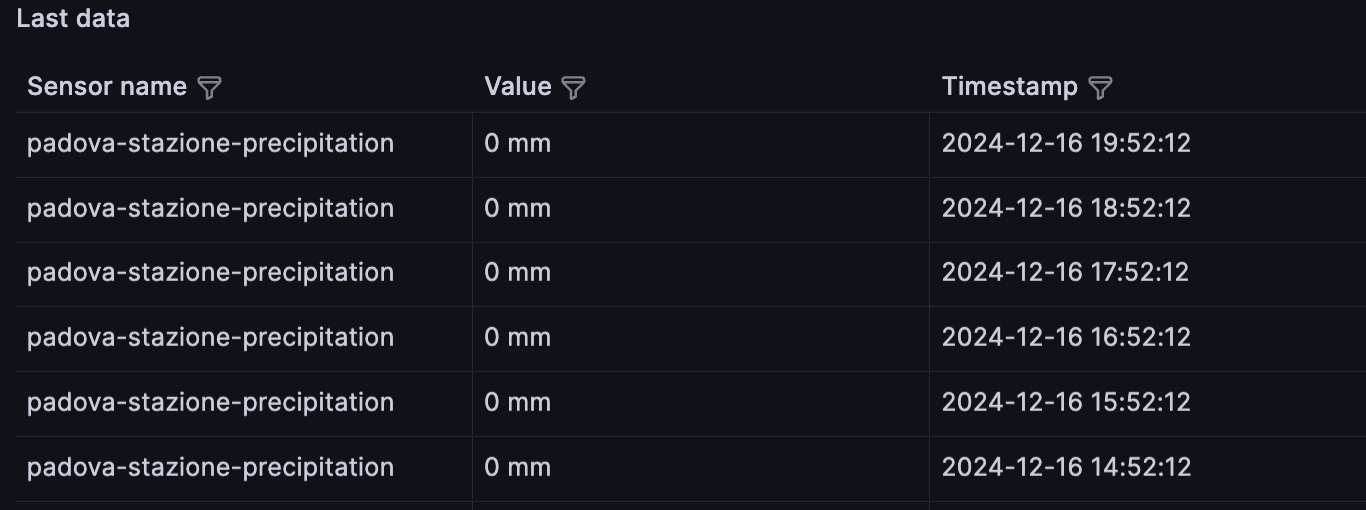
\includegraphics[width=0.7\textwidth]{manuale_utente/Rawdata/precipitation_table_rawdata.png}
            \captionof{figure}{Tabella dati raccolti Raw Data - Precipitation}
        \end{center}
        \item grafico a linee con lo storico dell'andamento delle precipitazioni;
        \begin{center}
            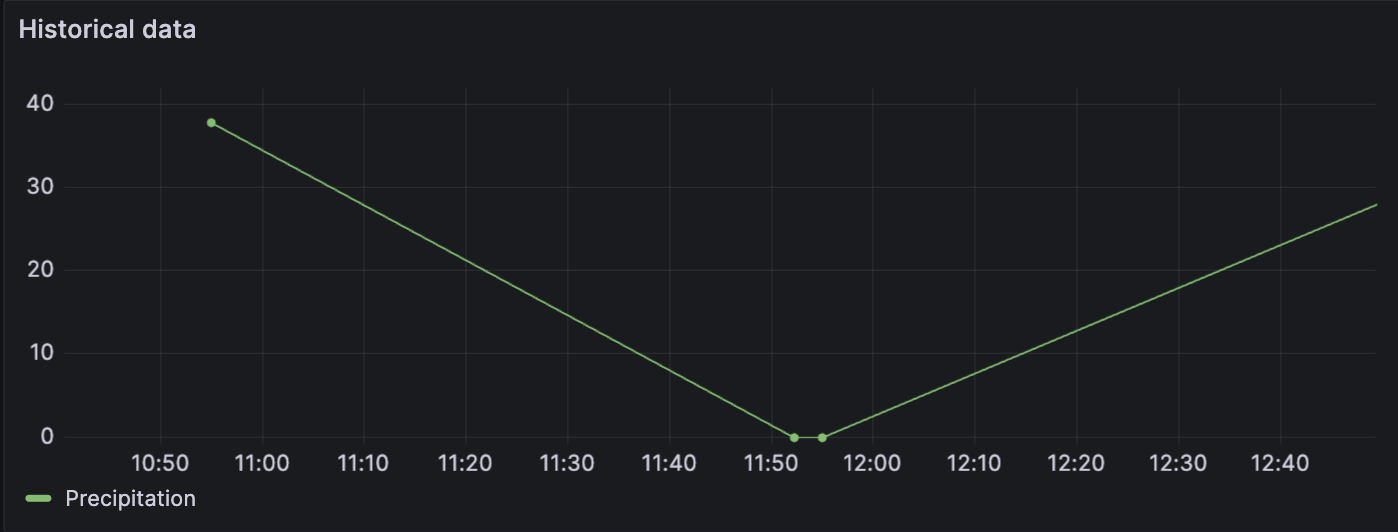
\includegraphics[width=0.7\textwidth]{manuale_utente/Rawdata/precipitation_rawdata.png}
            \captionof{figure}{Grafico precipitazione Raw Data - Precipitation}
        \end{center}
    \end{itemize}
    \item riga \textit{\textbf{River level}} contenente:
    \begin{itemize}
        \item tabella con gli ultimi dati raccolti;
        \begin{center}
            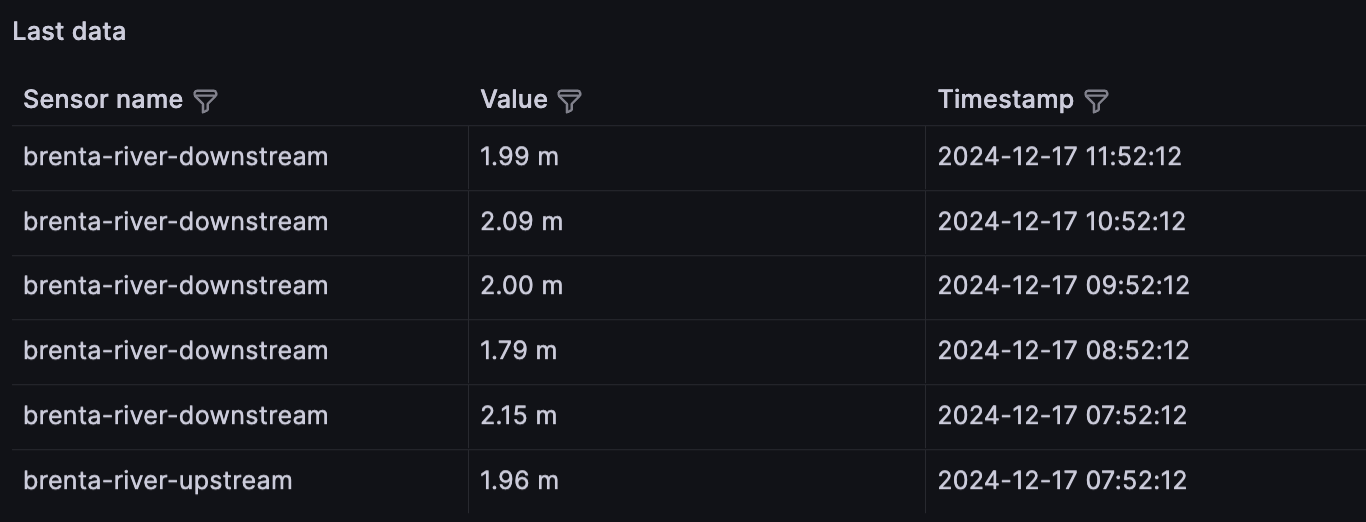
\includegraphics[width=0.7\textwidth]{manuale_utente/Rawdata/river_table_rawdata.png}
            \captionof{figure}{Tabella dati raccolti Raw Data - River level}
        \end{center}
        \item grafico a linee con lo storico dell'andamento del livello del fiume;
        \begin{center}
            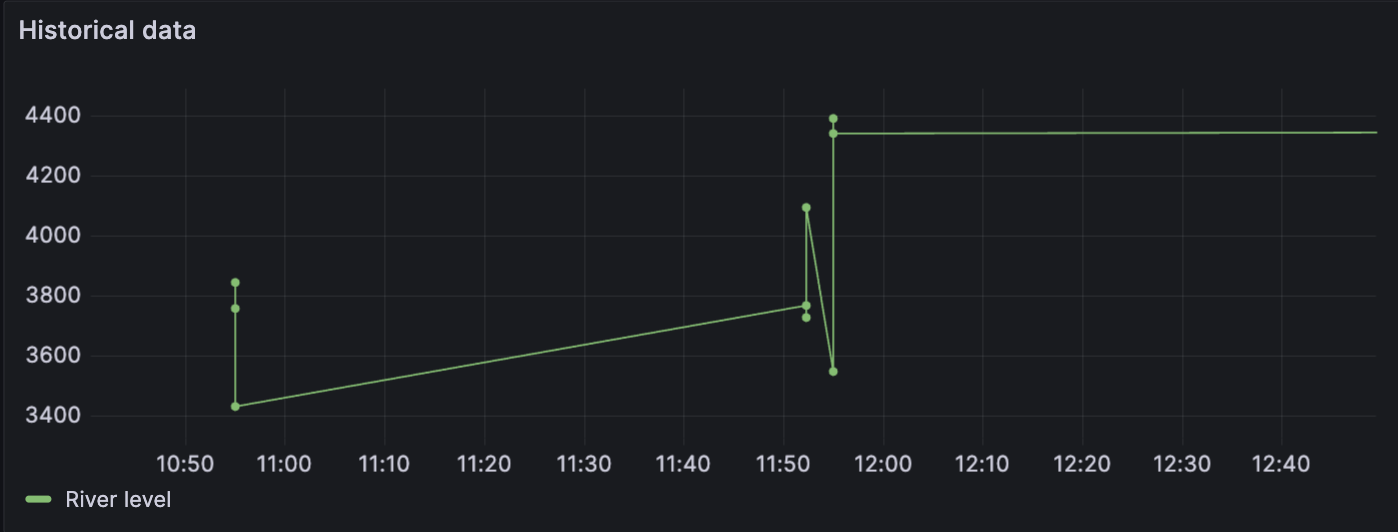
\includegraphics[width=0.7\textwidth]{manuale_utente/Rawdata/river_level_rawdata.png}
            \captionof{figure}{Grafico livello fiumi Raw Data - River level}
        \end{center}
    \end{itemize}
    \item riga \textit{\textbf{Recycling points}} contenente:
    \begin{itemize}
        \item tabella con gli ultimi dati raccolti;
        \begin{center}
            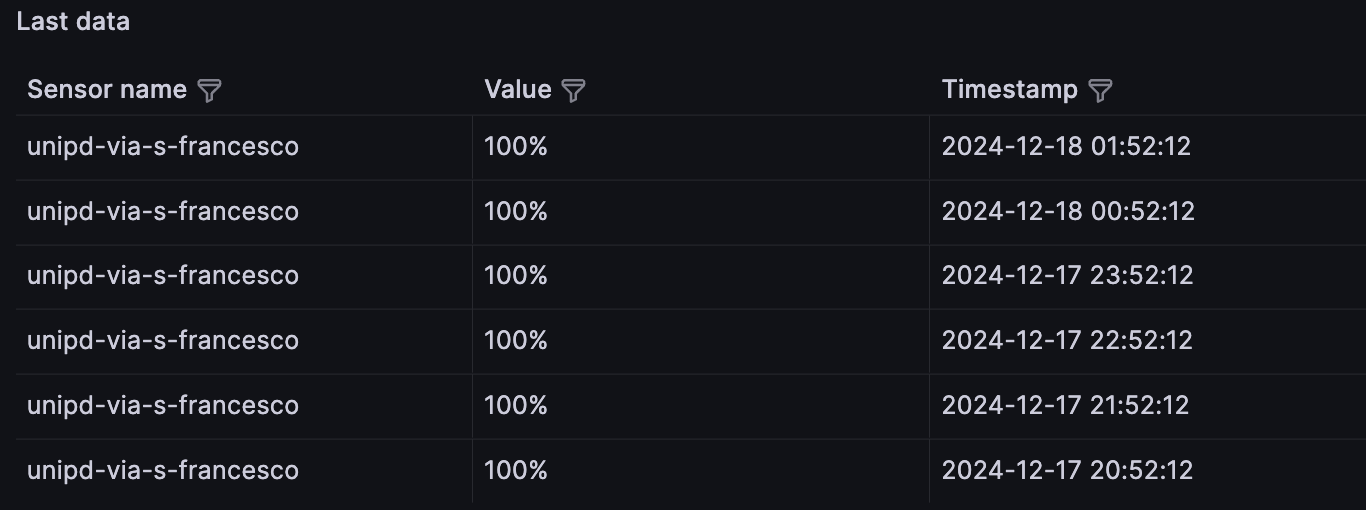
\includegraphics[width=0.7\textwidth]{manuale_utente/Rawdata/recycling_table_rawdata.png}
            \captionof{figure}{Tabella dati raccolti Raw Data - Recycling points}
        \end{center}
        \item grafico a linee con lo storico del riempimento delle isole ecologiche;
        \begin{center}
            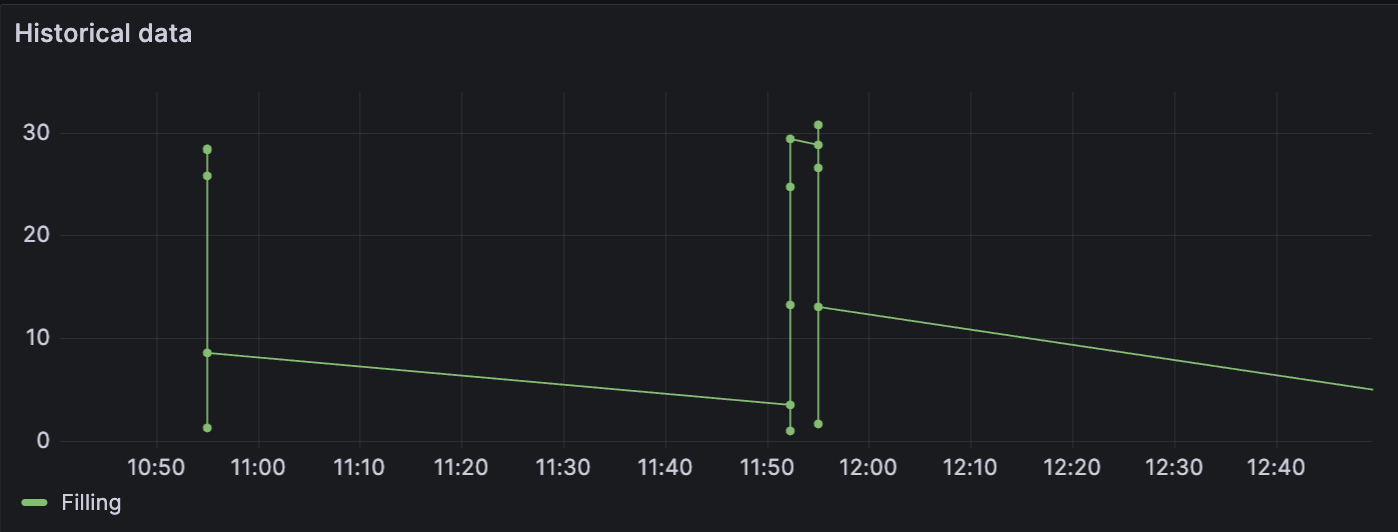
\includegraphics[width=0.7\textwidth]{manuale_utente/Rawdata/recycling_rawdata.png}
            \captionof{figure}{Grafico riempimento isole ecologiche Raw Data - Recycling points}
        \end{center}
    \end{itemize}
    \item riga \textit{\textbf{Traffic}} contenente:
    \begin{itemize}
        \item tabella con gli ultimi dati raccolti;
        \begin{center}
            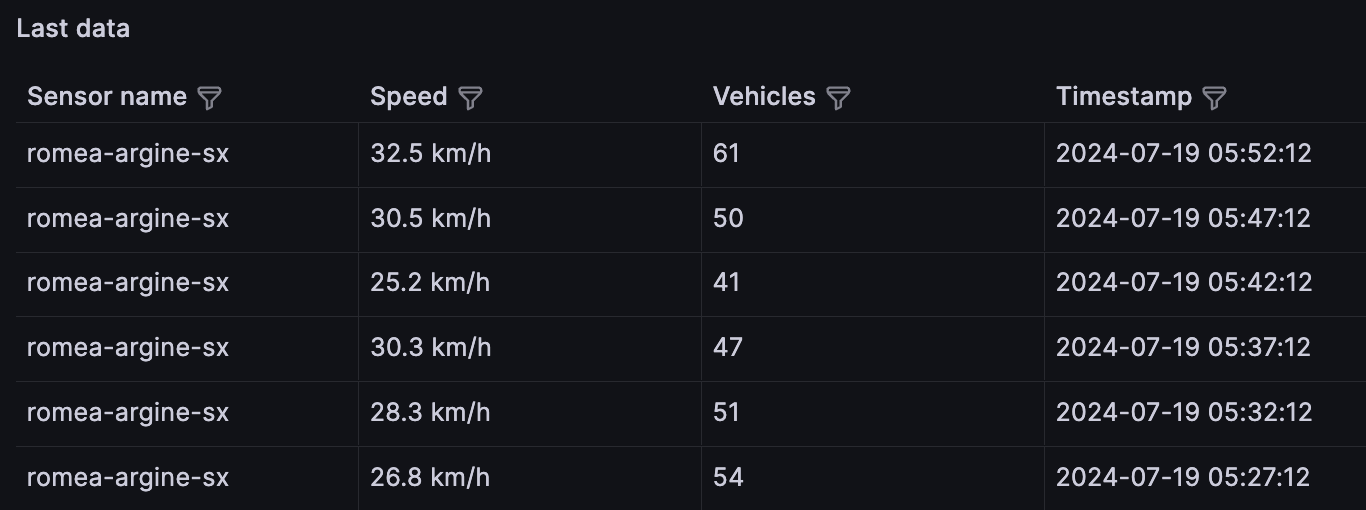
\includegraphics[width=0.7\textwidth]{manuale_utente/Rawdata/traffic_table_rawdata.png}
            \captionof{figure}{Tabella dati raccolti Raw Data - Traffic}
        \end{center}
        \item grafico a linee con lo storico del traffico;
        \begin{center}
            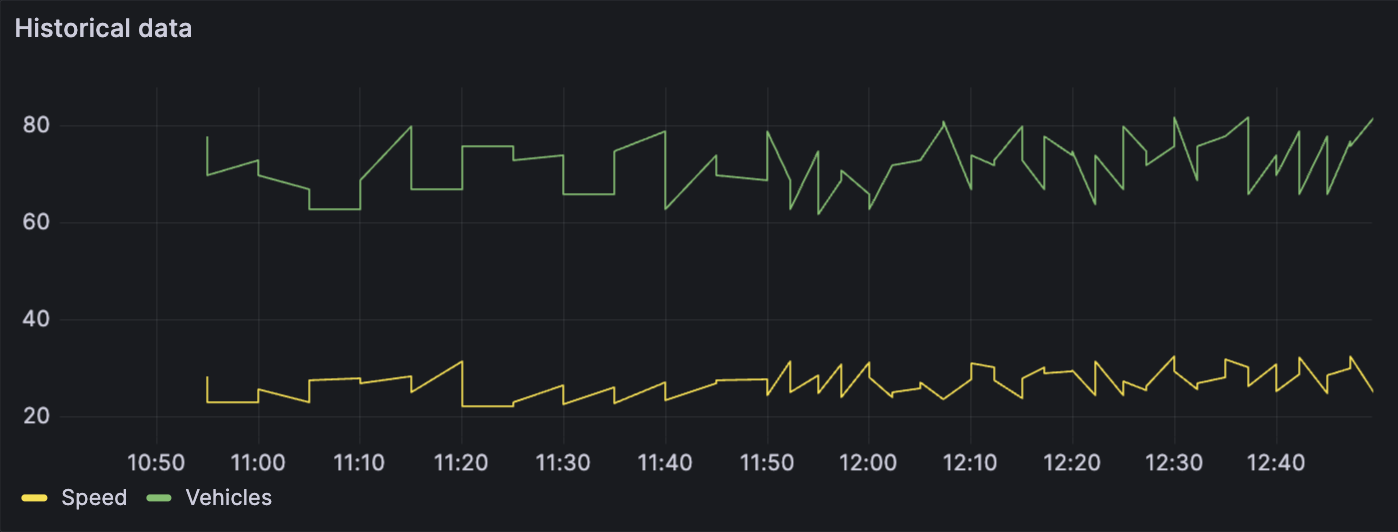
\includegraphics[width=0.7\textwidth]{manuale_utente/Rawdata/traffic_rawdata.png}
            \captionof{figure}{Grafico traffico Raw Data - Traffic}
        \end{center}
    \end{itemize}
\end{itemize}

\begin{center}
    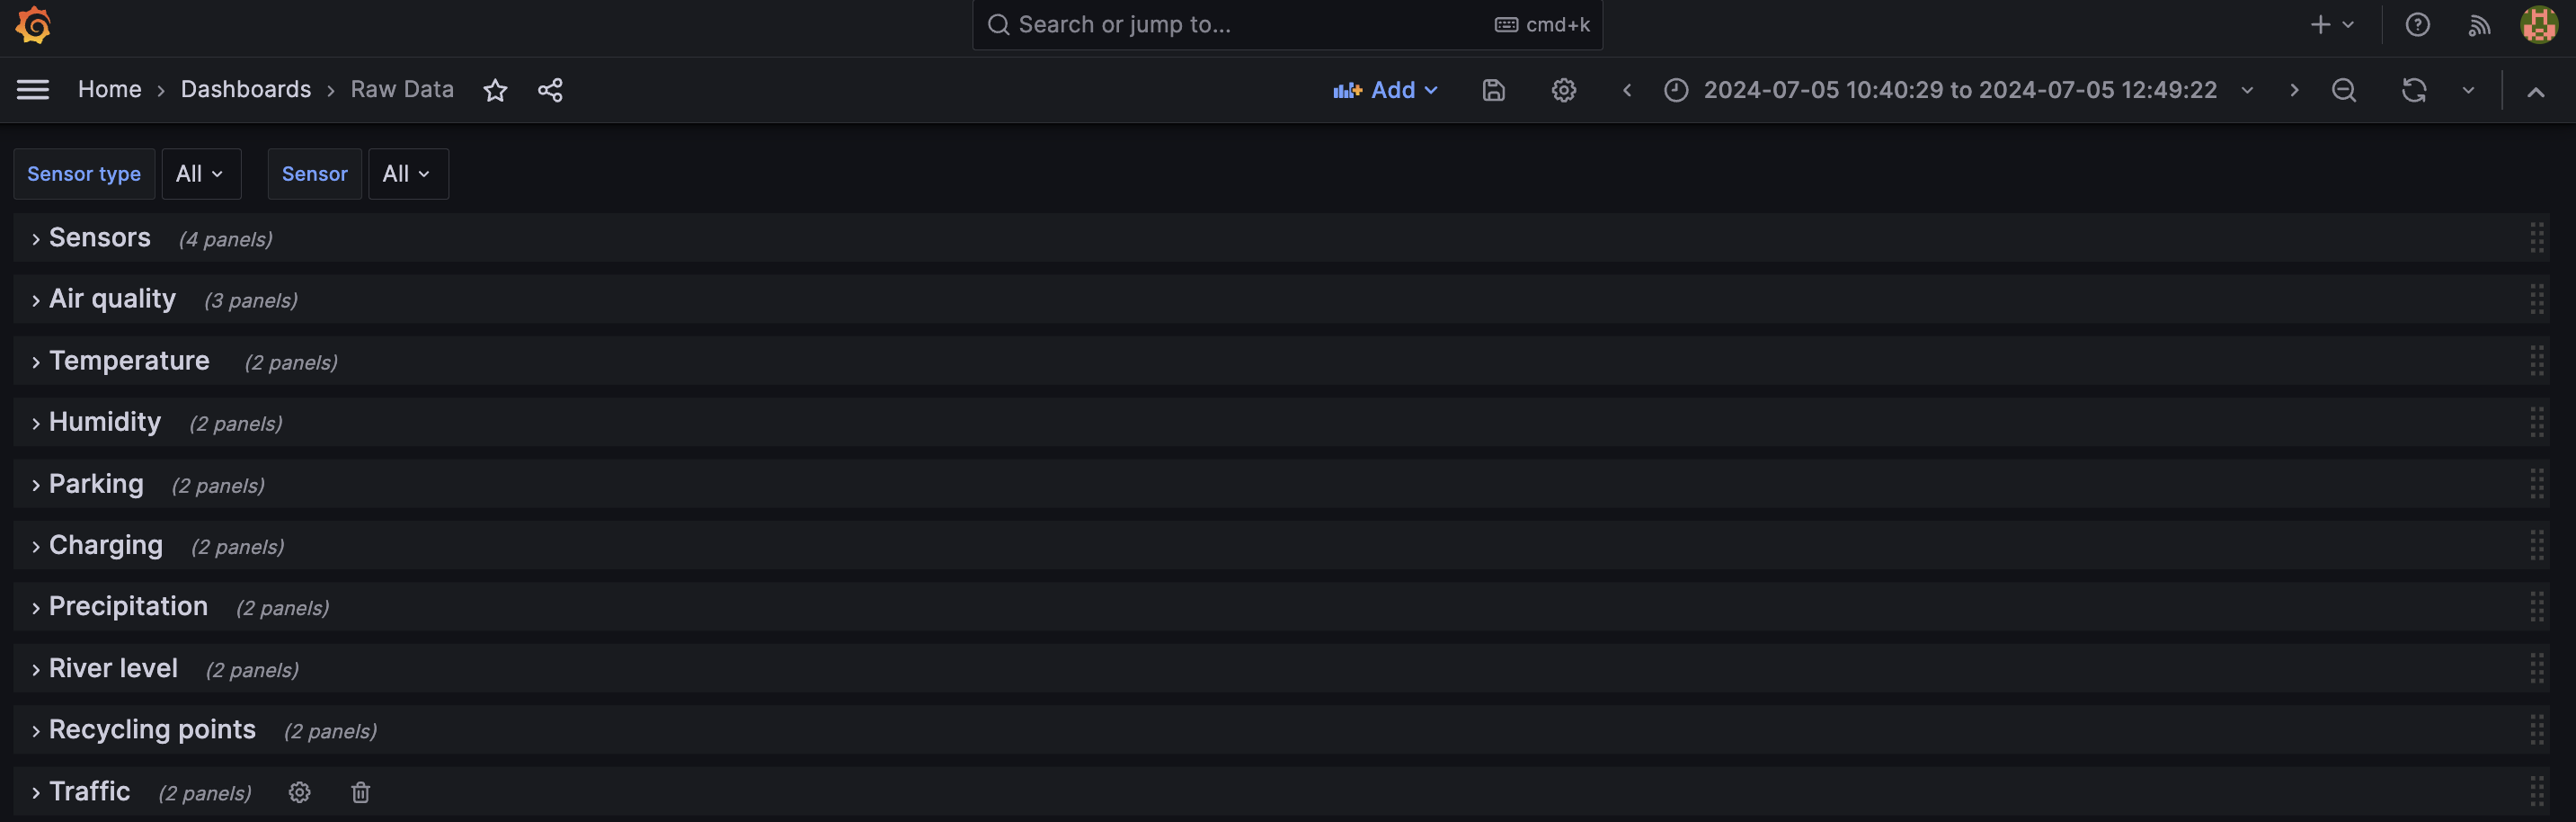
\includegraphics[width=\textwidth]{manuale_utente/Rawdata/rawdata_chiusa.png}
    \captionof{figure}{\href{https://7last.github.io/docs/pb/documentazione-interna/glossario\#dashboard}{Dashboard\textsubscript{G}} generale con le righe chiuse}
\end{center}

\begin{center}
    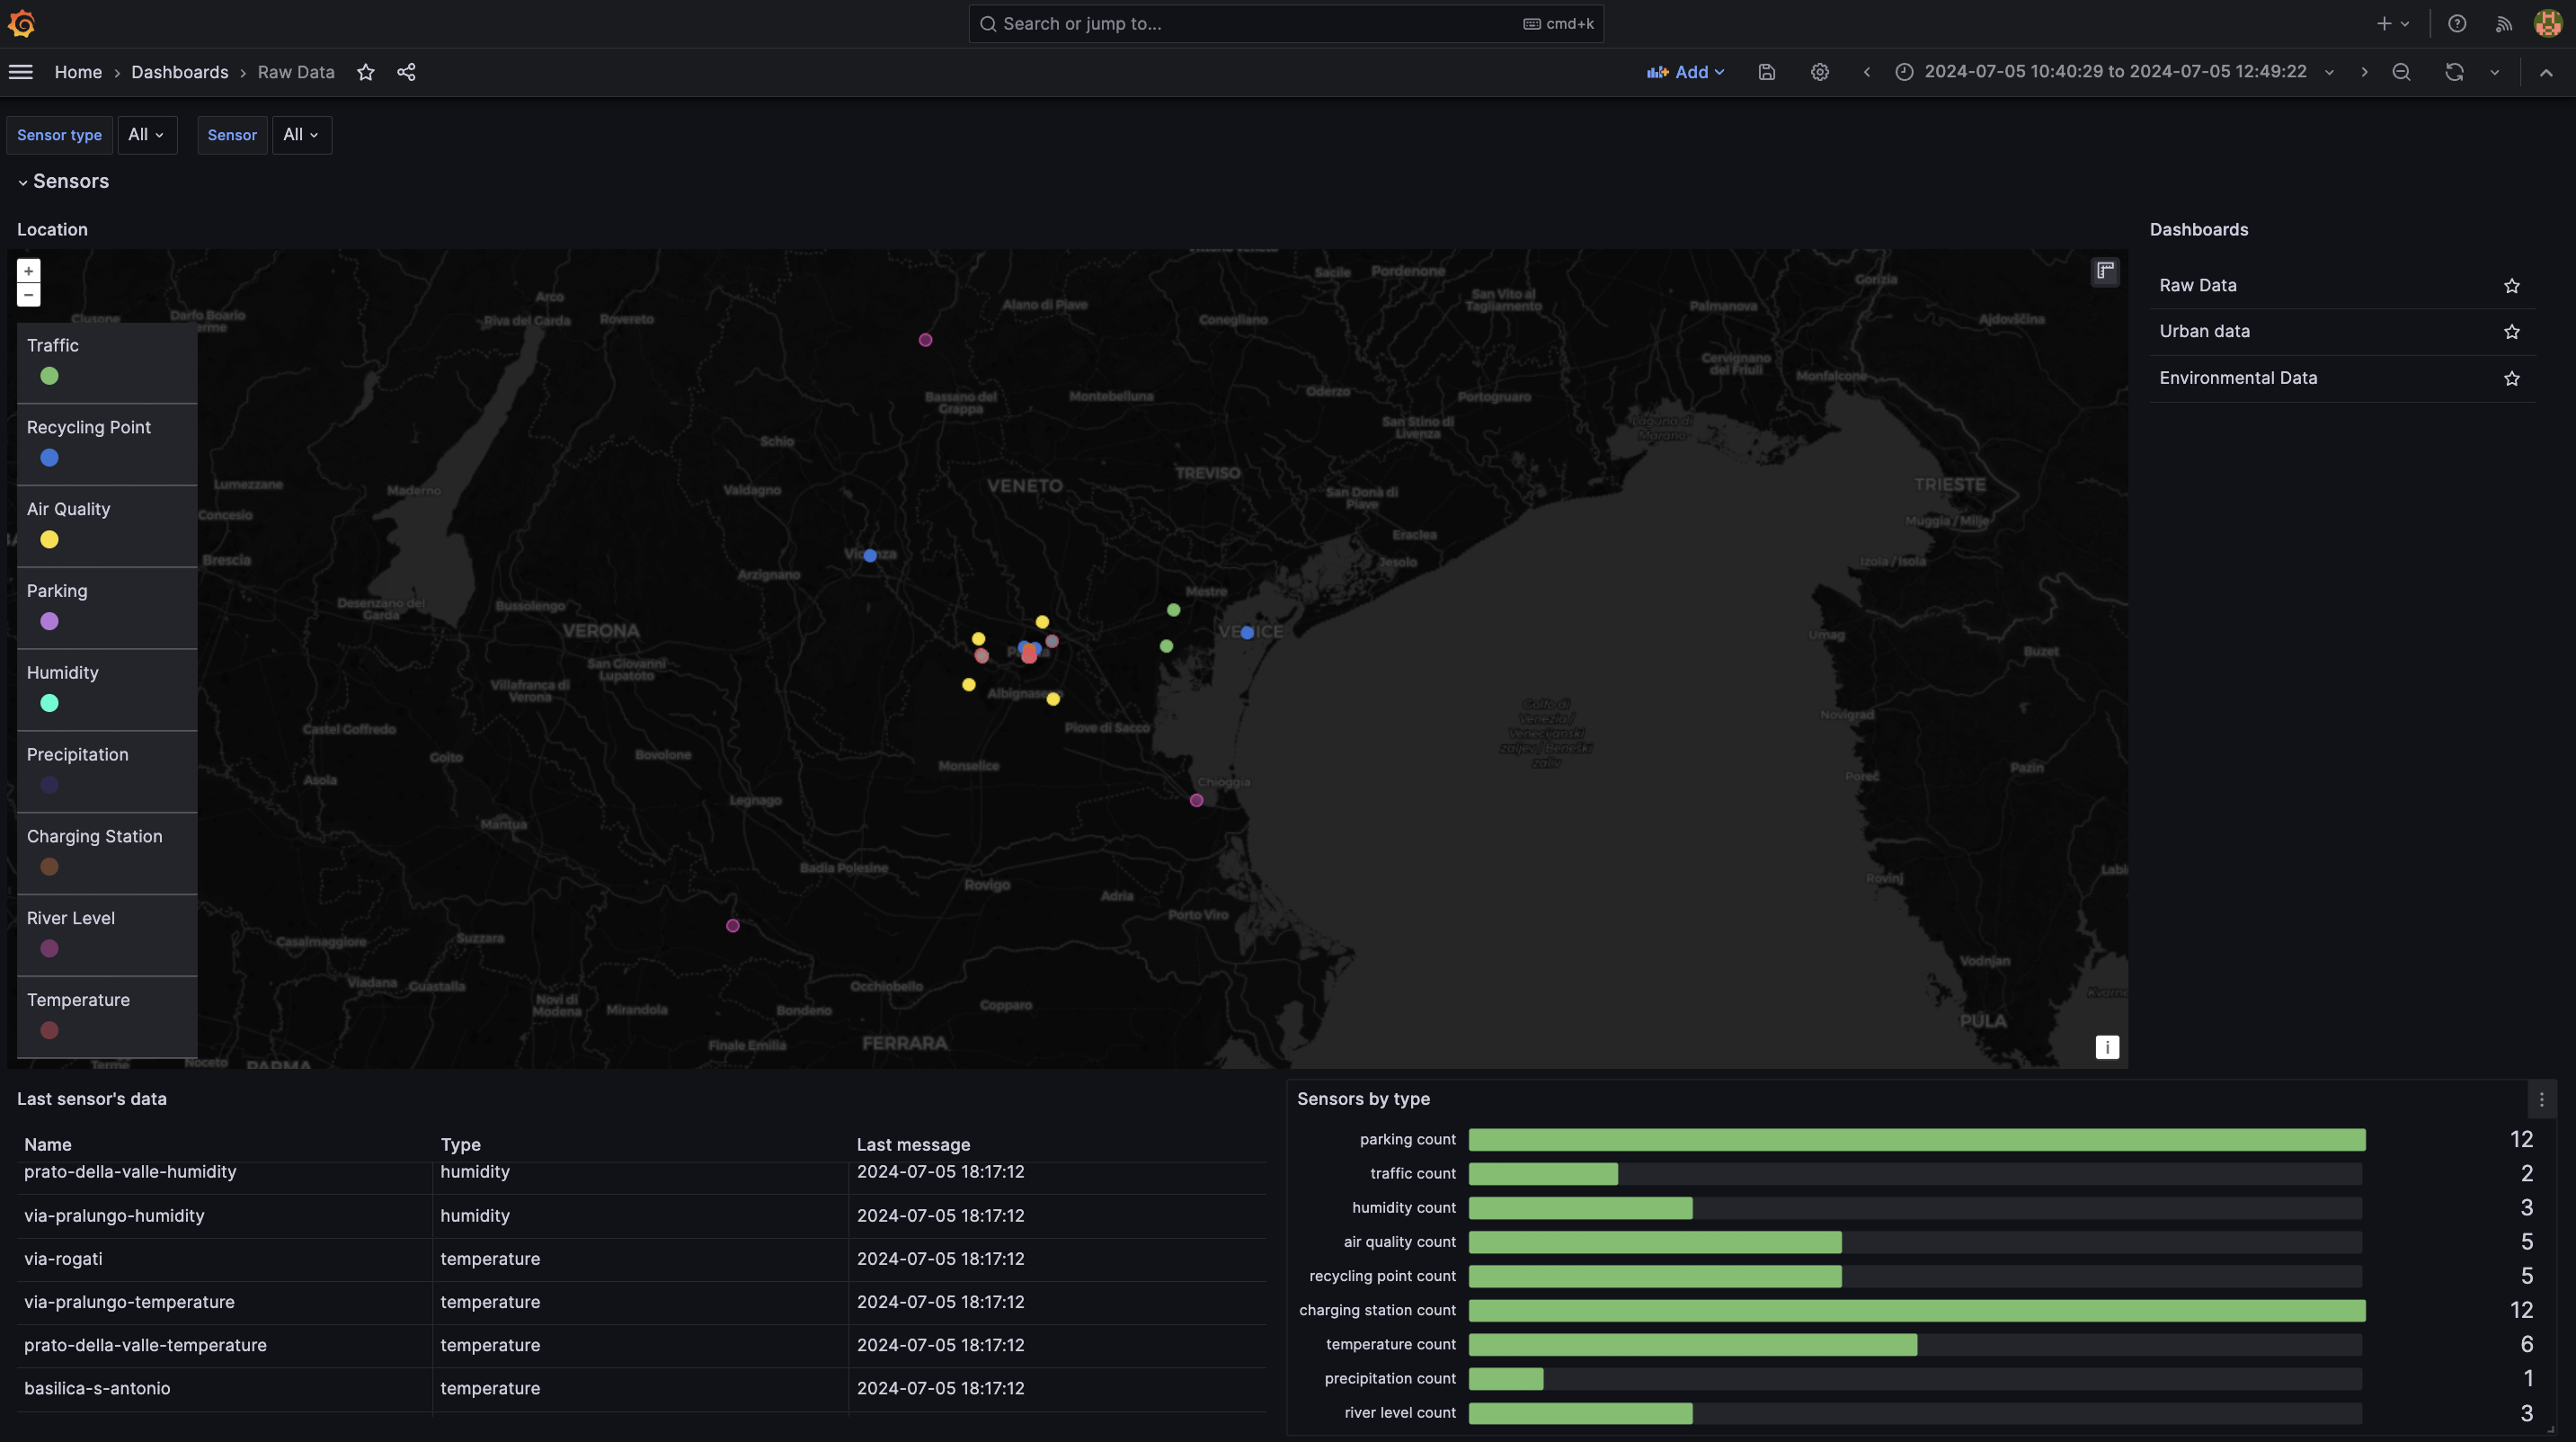
\includegraphics[width=\textwidth]{manuale_utente/Rawdata/rawdata_aperta.png}
    \captionof{figure}{\href{https://7last.github.io/docs/pb/documentazione-interna/glossario\#dashboard}{Dashboard\textsubscript{G}} generale con \textit{Sensor} aperta}
\end{center}


\newpage
\subsubsection{Environmental Data}
Tale \href{https://7last.github.io/docs/pb/documentazione-interna/glossario\#dashboard}{\textit{dashboard}\textsubscript{G}} offre una visualizzazione dettagliata delle informazioni sui sensori ambientali ubicati in specifiche aree. Comprende grafici interattivi per monitorare l'andamento delle misurazioni nel tempo e statistiche riassuntive per una panoramica immediata. Organizzata dall'alto verso il basso e da sinistra verso destra, è composta da:
\begin{itemize}
    \item filtro per visualizzare i sensori di preferenza;
    \begin{center}
        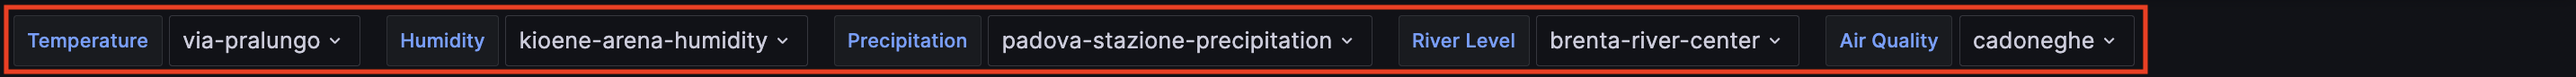
\includegraphics[width=0.7\textwidth]{manuale_utente/Environmental/filter.png}
        \captionof{figure}{Filtro \href{https://7last.github.io/docs/pb/documentazione-interna/glossario\#dashboard}{\textit{dashboard}\textsubscript{G}} \textit{Environmental Data}}
    \end{center}
    \item riga \textit{\textbf{Temperature}} contenente:
    \begin{itemize}
        \item mappa dei sensori; %TODO mettere immagine mappa temperatura "environmental data"
        \item grafico a linee con l'andamento della temperatura nel tempo; %TODO mettere immagine grafico temperatura "environmental data"
        \item grafico a barre con la media giornaliera e settimanale della temperatura;
        \begin{center}
            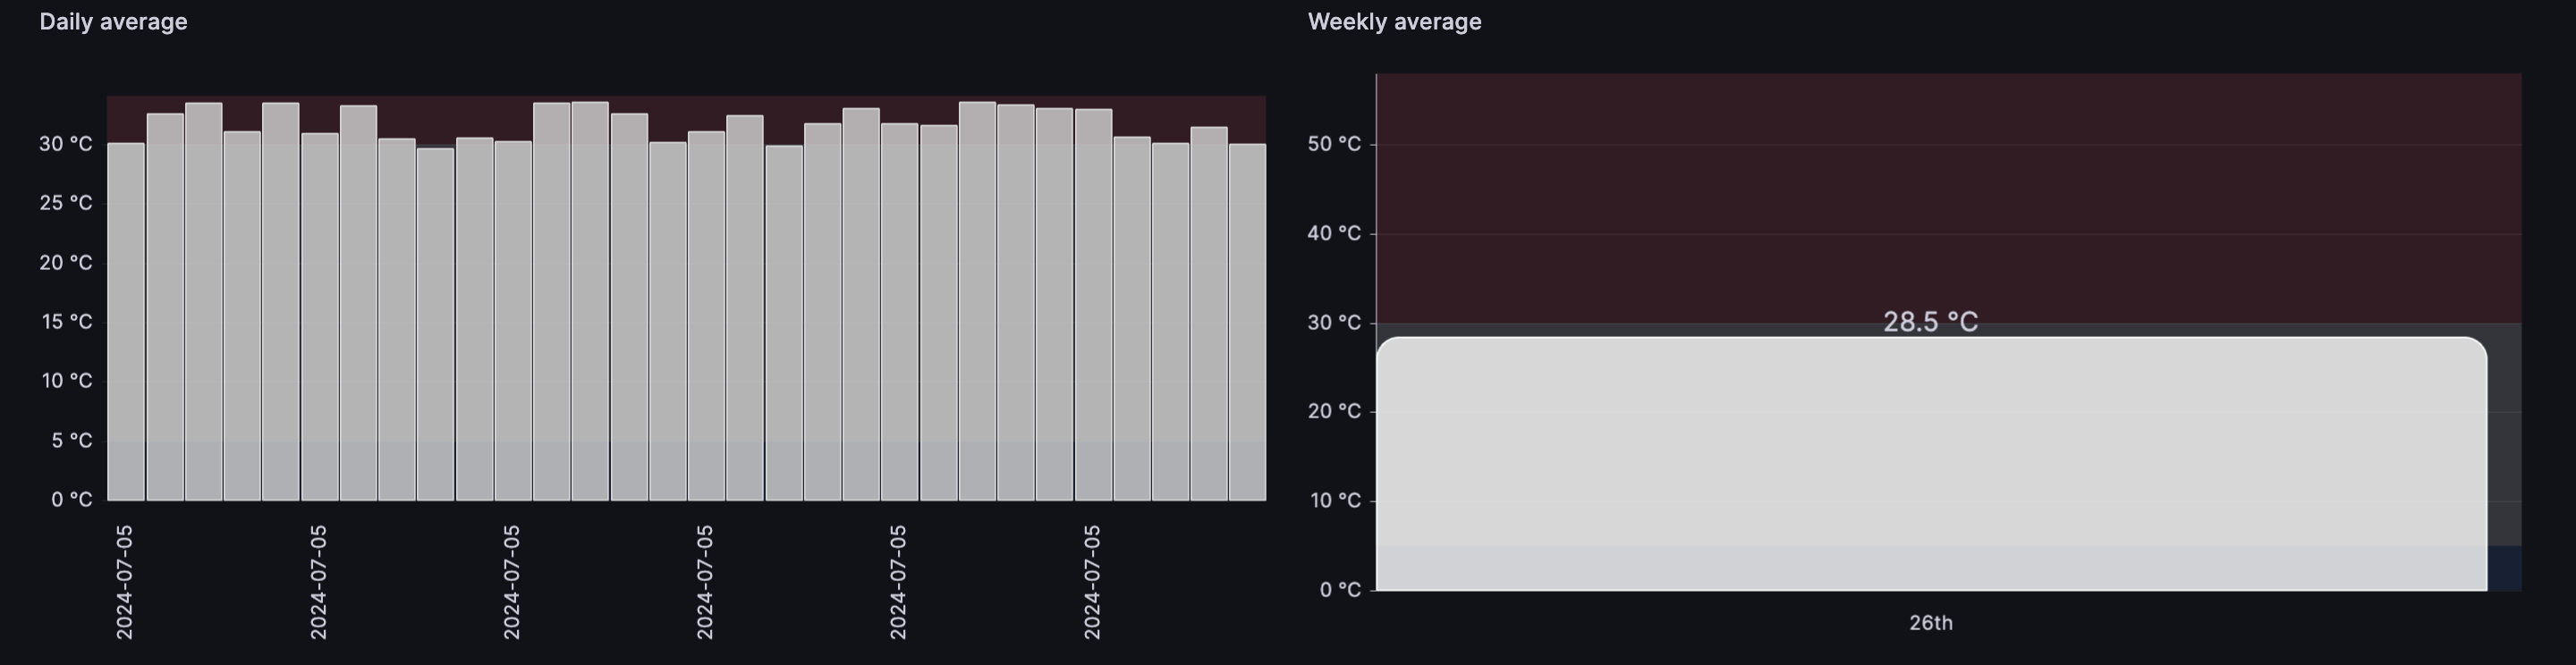
\includegraphics[width=0.7\textwidth]{manuale_utente/Environmental/avg_temp_env.png}
            \captionof{figure}{Grafico temperatura giornaliera e settimanale \href{https://7last.github.io/docs/pb/documentazione-interna/glossario\#dashboard}{\textit{dashboard}\textsubscript{G}} \textit{Environmental Data}}
        \end{center}
        \item grafico Gauge con la temperatura minima, massima e media;
        \begin{center}
            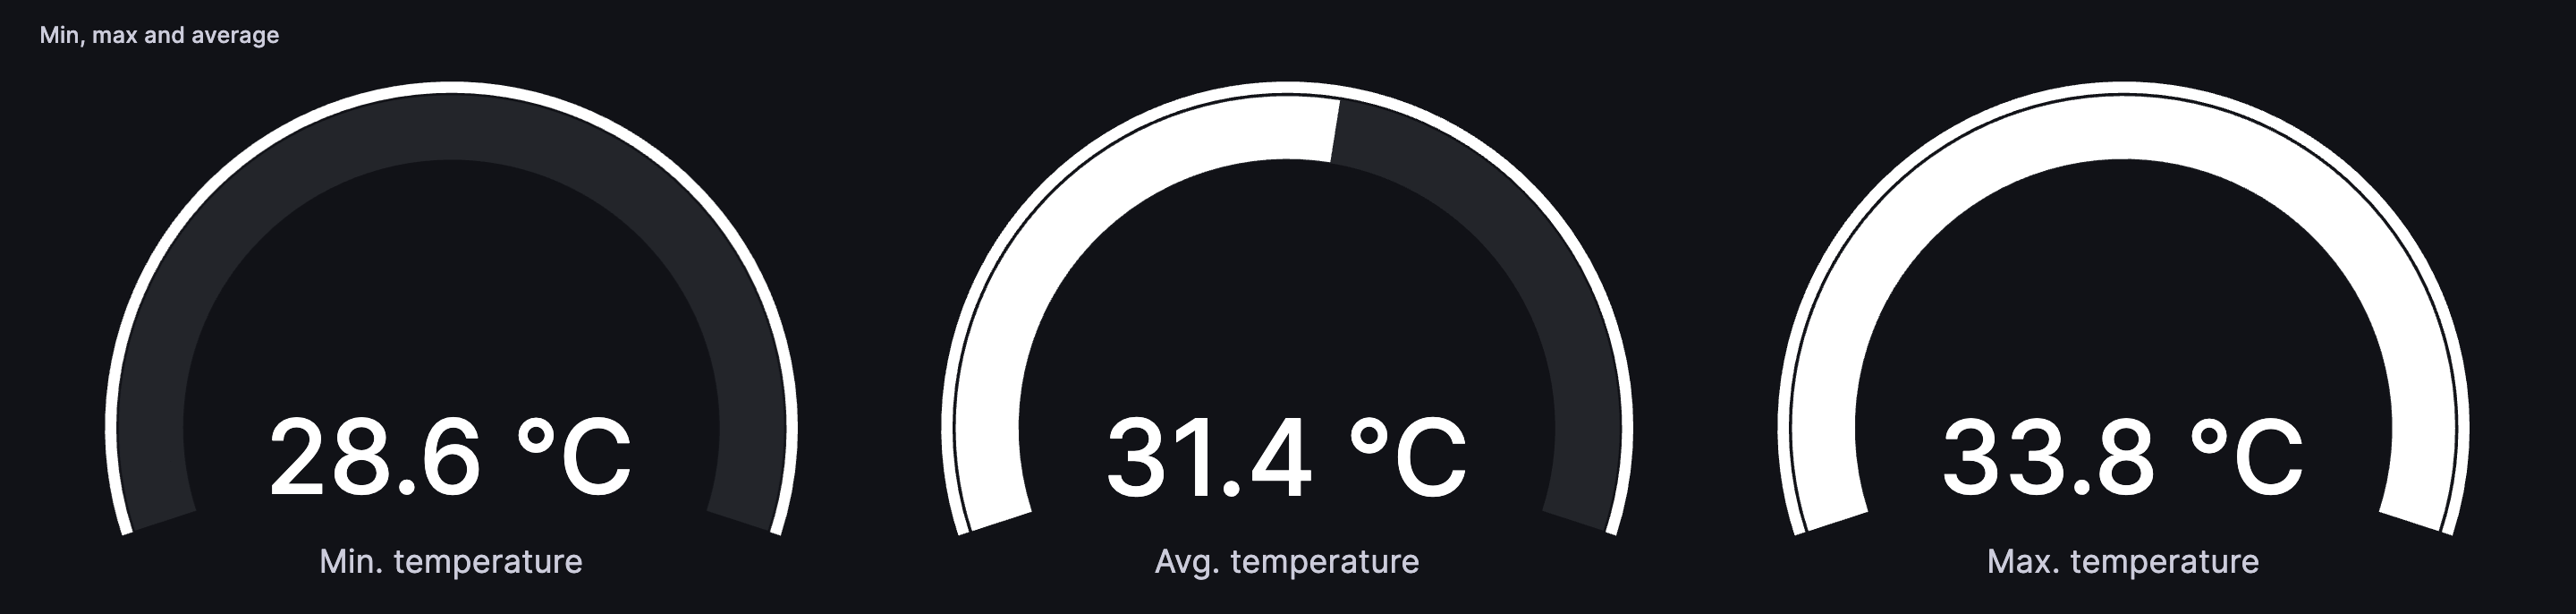
\includegraphics[width=0.7\textwidth]{manuale_utente/Environmental/min_temperature_env.png}
            \captionof{figure}{Grafico temperatura minima, massima e media \href{https://7last.github.io/docs/pb/documentazione-interna/glossario\#dashboard}{\textit{dashboard}\textsubscript{G}} \textit{Environmental Data}}
        \end{center}
    \end{itemize}

    \item riga \textit{\textbf{Humidity}} contenente:
    \begin{itemize}
        \item mappa dei sensori;
        \begin{center}
            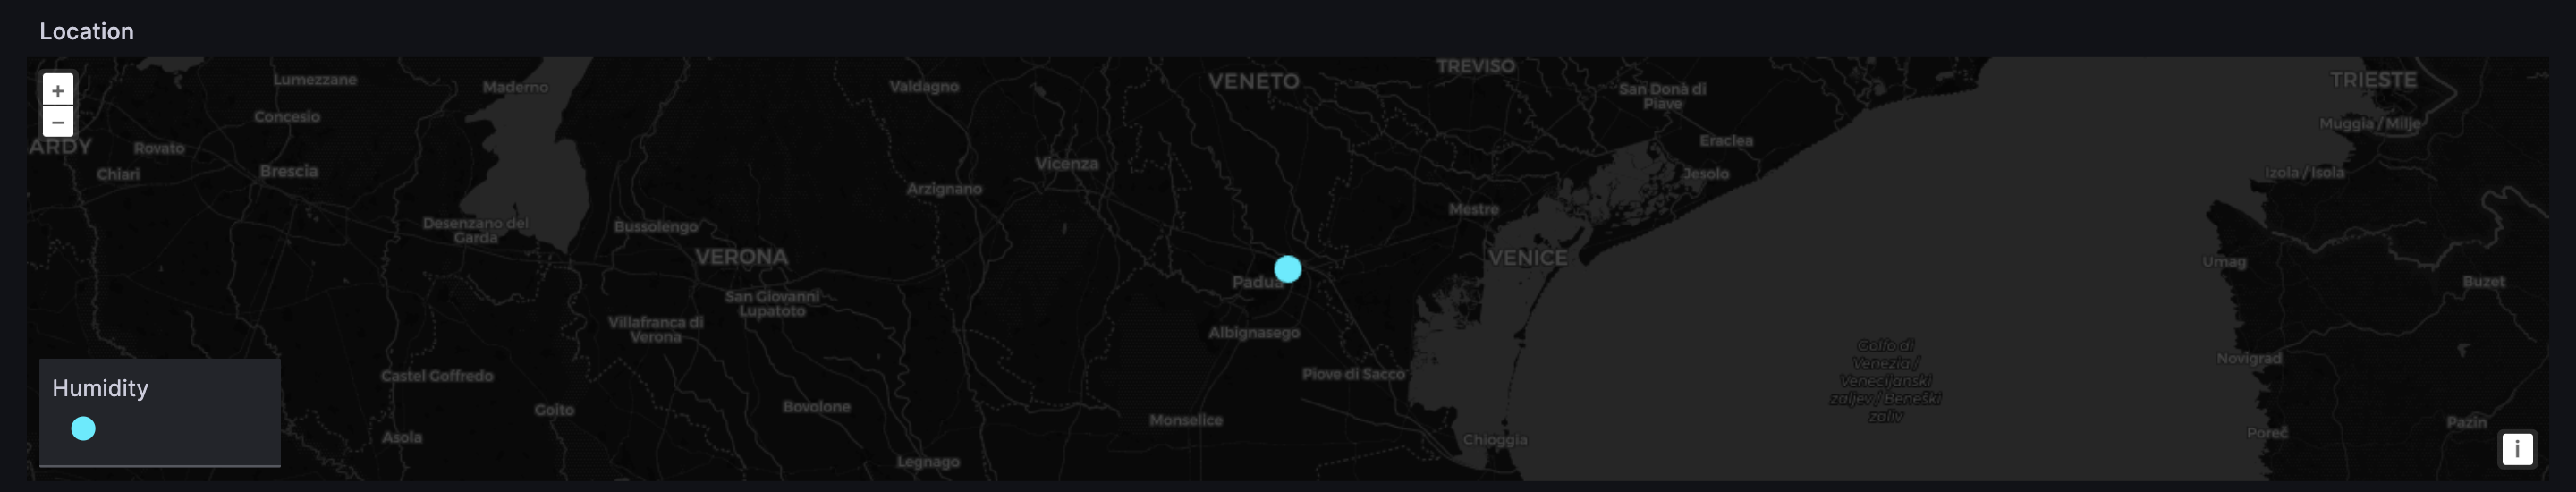
\includegraphics[width=0.7\textwidth]{manuale_utente/Environmental/map_hum_env.png}
            \captionof{figure}{Grafico mappa umidità \href{https://7last.github.io/docs/pb/documentazione-interna/glossario\#dashboard}{\textit{dashboard}\textsubscript{G}} \textit{Environmental Data}}
        \end{center}
        \item grafico a barre con la media giornaliera e settimanale dell'umidità;
        \begin{center}
            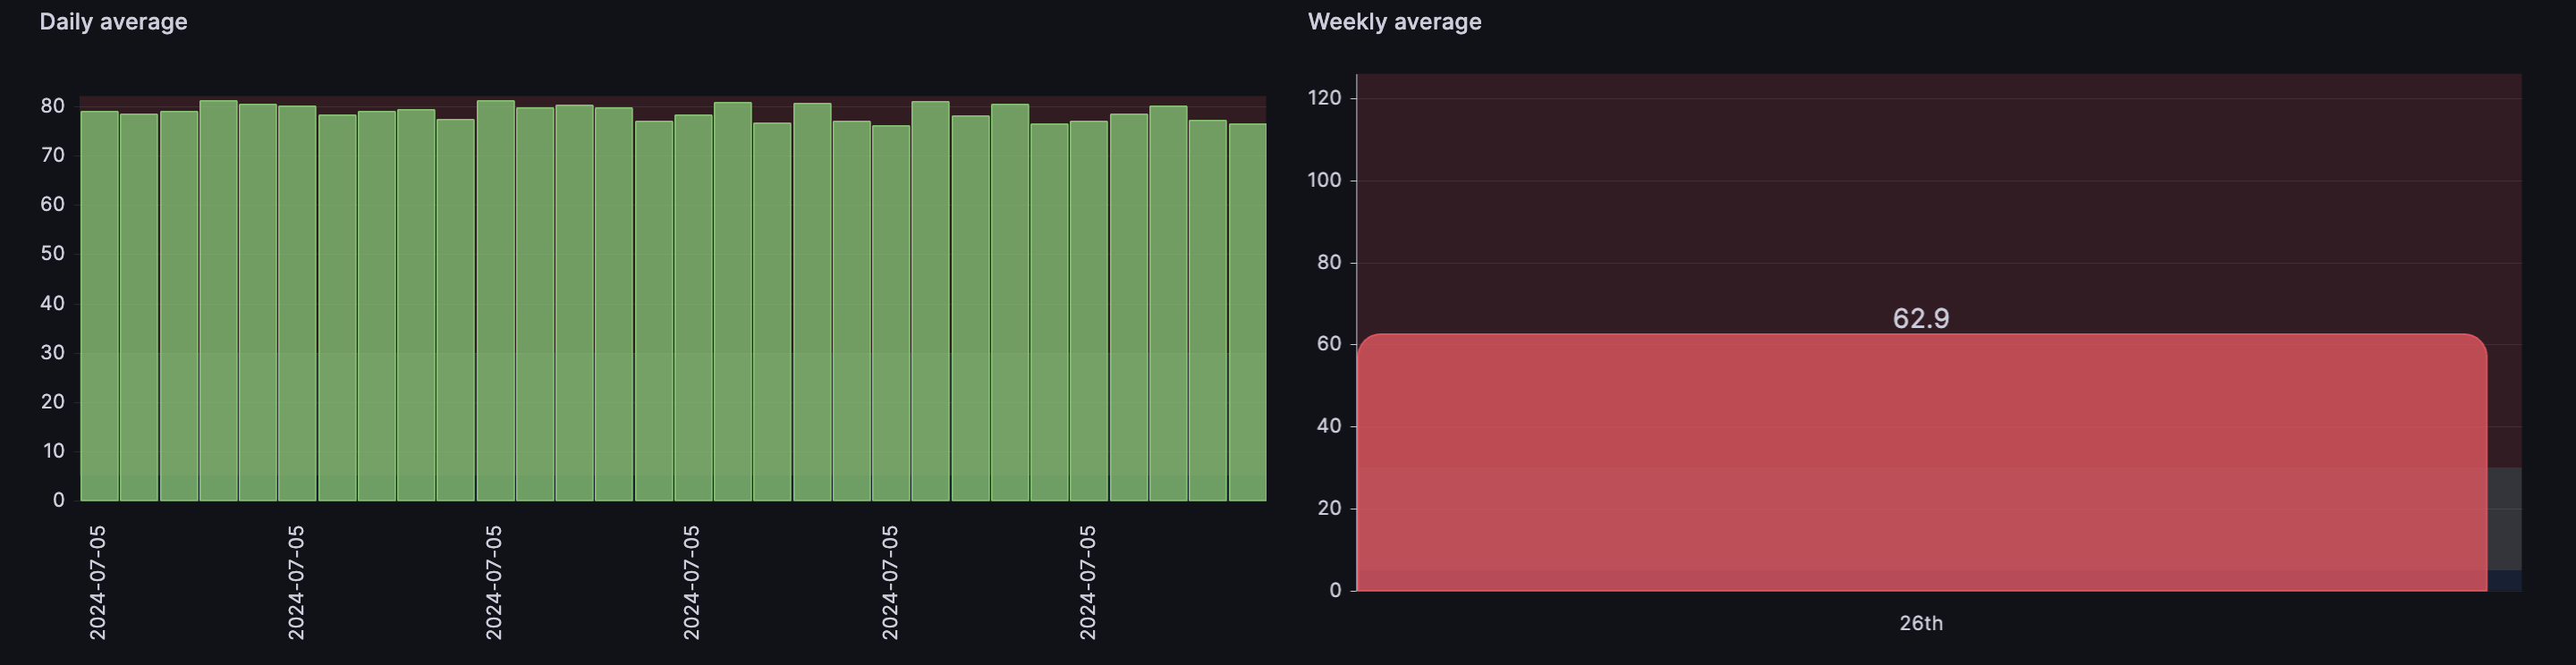
\includegraphics[width=0.7\textwidth]{manuale_utente/Environmental/avg_hum_env.png}
            \captionof{figure}{Grafico umidità settimanale \href{https://7last.github.io/docs/pb/documentazione-interna/glossario\#dashboard}{\textit{dashboard}\textsubscript{G}} \textit{Environmental Data}}
        \end{center}
        \item grafico Gauge con l'umidità minima, massima e media;
        \begin{center}
            \includegraphics[width=0.7\textwidth]{manuale_utente/Environmental/min_hum_env.png}
            \captionof{figure}{Grafico umidità minima, massima e media \href{https://7last.github.io/docs/pb/documentazione-interna/glossario\#dashboard}{\textit{dashboard}\textsubscript{G}} \textit{Environmental Data}}
        \end{center}
    \end{itemize}

    \item riga \textit{\textbf{Precipitation}} contenente:
    \begin{itemize}
        \item mappa dei sensori;
        \begin{center}
            \includegraphics[width=0.7\textwidth]{manuale_utente/Environmental/map_prec_env.png}
            \captionof{figure}{Grafico mappa sensori precipitazioni \href{https://7last.github.io/docs/pb/documentazione-interna/glossario\#dashboard}{\textit{dashboard}\textsubscript{G}} \textit{Environmental Data}}
        \end{center}
        \item grafico a linee con la media oraria e grafico a barre con la media giornaliera delle precipitazioni;
        \begin{center}
            \includegraphics[width=0.7\textwidth]{manuale_utente/Environmental/avg_prec_env.png}
            \captionof{figure}{Grafico precipitazioni orarie e giornaliere \href{https://7last.github.io/docs/pb/documentazione-interna/glossario\#dashboard}{\textit{dashboard}\textsubscript{G}} \textit{Environmental Data}}
        \end{center}
        \item grafico a linee con la media mensile e grafico a barre con la media annuale delle precipitazioni;
        \begin{center}
            \includegraphics[width=0.7\textwidth]{manuale_utente/Environmental/avg_prec_month_env.png}
            \captionof{figure}{Grafico precipitazioni mensili e annuali \href{https://7last.github.io/docs/pb/documentazione-interna/glossario\#dashboard}{\textit{dashboard}\textsubscript{G}} \textit{Environmental Data}}
        \end{center}
        \item grafico Gauge con la precipitazione minima, massima e media;
        \begin{center}
            \includegraphics[width=0.7\textwidth]{manuale_utente/Environmental/min_prec_env.png}
            \captionof{figure}{Grafico precipitazione minima, massima e media \href{https://7last.github.io/docs/pb/documentazione-interna/glossario\#dashboard}{\textit{dashboard}\textsubscript{G}} \textit{Environmental Data}}
        \end{center}
    \end{itemize}

    \item riga \textit{\textbf{River level}} contenente:
    \begin{itemize}
        \item mappa dei sensori;
        \begin{center}
            \includegraphics[width=0.7\textwidth]{manuale_utente/Environmental/map_river_env.png}
            \captionof{figure}{Grafico mappa sensori livello fiumi \href{https://7last.github.io/docs/pb/documentazione-interna/glossario\#dashboard}{\textit{dashboard}\textsubscript{G}} \textit{Environmental Data}}
        \end{center}
        \item grafico a linee con la media oraria e grafico a barre con la media giornaliera delle livello fiumi;
        \begin{center}
            \includegraphics[width=0.7\textwidth]{manuale_utente/Environmental/avg_river_env.png}
            \captionof{figure}{Grafico livello fiumi orari e giornalieri \href{https://7last.github.io/docs/pb/documentazione-interna/glossario\#dashboard}{\textit{dashboard}\textsubscript{G}} \textit{Environmental Data}}
        \end{center}
        \item grafico a linee con la media mensile e grafico a barre con la media annuale del livello fiumi;
        \begin{center}
            \includegraphics[width=0.7\textwidth]{manuale_utente/Environmental/avg_river_month_env.png}
            \captionof{figure}{Grafico livello fiumi mensili e annuali \href{https://7last.github.io/docs/pb/documentazione-interna/glossario\#dashboard}{\textit{dashboard}\textsubscript{G}} \textit{Environmental Data}}
        \end{center}
        \item grafico Gauge con il livello dei fiumi minimo, massimo e medio;
        \begin{center}
            \includegraphics[width=0.7\textwidth]{manuale_utente/Environmental/min_river_env.png}
            \captionof{figure}{Grafico livello fiume minimo, massimo e medio \href{https://7last.github.io/docs/pb/documentazione-interna/glossario\#dashboard}{\textit{dashboard}\textsubscript{G}} \textit{Environmental Data}}
        \end{center}
    \end{itemize}

    \item riga \textit{\textbf{Air quality}} contenente:
    \begin{itemize}
        \item mappa qualità dell'aria;
        \begin{center}
            \includegraphics[width=0.7\textwidth]{manuale_utente/Environmental/map_air_env.png}
            \captionof{figure}{Mappa qualità dell'aria \href{https://7last.github.io/docs/pb/documentazione-interna/glossario\#dashboard}{\textit{dashboard}\textsubscript{G}} \textit{Environmental Data}}
        \end{center}
        \item grafico Gauge con l'indice europeo della qualità dell'aria e grafico a barre con la media degli agenti inquinanti;
        \begin{center}
            \includegraphics[width=0.7\textwidth]{manuale_utente/Environmental/air_index_env.png}
            \captionof{figure}{Indice qualità aria e quantità agenti inquinanti \href{https://7last.github.io/docs/pb/documentazione-interna/glossario\#dashboard}{\textit{dashboard}\textsubscript{G}} \textit{Environmental Data}}
        \end{center}
        \item grafico a barre con gli agenti inquinanti;
        \begin{center}
            \includegraphics[width=0.7\textwidth]{manuale_utente/Environmental/air_quality_env.png}
            \captionof{figure}{Inquinanti \href{https://7last.github.io/docs/pb/documentazione-interna/glossario\#dashboard}{\textit{dashboard}\textsubscript{G}} \textit{Environmental Data}}
        \end{center}
    \end{itemize}
\end{itemize}

\subsubsection{Urban Data}
Tale \href{https://7last.github.io/docs/pb/documentazione-interna/glossario\#dashboard}{\textit{dashboard}\textsubscript{G}} offre una visualizzazione dettagliata delle informazioni sui sensori urbani ubicati in specifiche aree. Comprende grafici interattivi per monitorare l'andamento delle misurazioni nel tempo e statistiche riassuntive per una panoramica immediata. Organizzata dall'alto verso il basso e da sinistra verso destra, è composta da:
\begin{itemize}
    \item filtro per visualizzare i sensori di preferenza;
    \begin{center}
        \includegraphics[width=0.7\textwidth]{manuale_utente/Urban/filter.png}
        \captionof{figure}{Filtro \href{https://7last.github.io/docs/pb/documentazione-interna/glossario\#dashboard}{\textit{dashboard}\textsubscript{G}} \textit{Urban Data}}
    \end{center}
    \item riga \textit{\textbf{Charging}} contenente:
    \begin{itemize}
        \item mappa dei sensori;
        \begin{center}
            \includegraphics[width=0.7\textwidth]{manuale_utente/Urban/map_charging.png}
            \captionof{figure}{Mappa sensori colonnine di ricarica \href{https://7last.github.io/docs/pb/documentazione-interna/glossario\#dashboard}{\textit{dashboard}\textsubscript{G}} \textit{Urban Data}}
        \end{center}
        \item grafico a barre orizzontali per il tempo totale di occupazione delle colonnine di ricarica e grafico a torta per l'occupazione in tempo reale delle stesse;
        \begin{center}
            \includegraphics[width=0.7\textwidth]{manuale_utente/Urban/graphs_charging.png}
            \captionof{figure}{Grafici occupazione colonnine di ricarica \href{https://7last.github.io/docs/pb/documentazione-interna/glossario\#dashboard}{\textit{dashboard}\textsubscript{G}} \textit{Urban Data}}
        \end{center}
        \item grafico \href{https://7last.github.io/docs/pb/documentazione-interna/glossario\#time-series}{time series\textsubscript{G}} e grafico Gauge per l'efficienza delle colonnine di ricarica;
        \begin{center}
            \includegraphics[width=0.7\textwidth]{manuale_utente/Urban/whole.png}
            \captionof{figure}{Grafici efficienza colonnine di ricarica \href{https://7last.github.io/docs/pb/documentazione-interna/glossario\#dashboard}{\textit{dashboard}\textsubscript{G}} \textit{Urban Data}}
        \end{center}
        \item grafico \textit{Canvas} per rappresentare la colonnina più efficiente e quella meno efficiente;
        \begin{center}
            \includegraphics[width=0.7\textwidth]{manuale_utente/Urban/efficiency.png}
            \captionof{figure}{Grafici efficienza colonnine di ricarica \href{https://7last.github.io/docs/pb/documentazione-interna/glossario\#dashboard}{\textit{dashboard}\textsubscript{G}} \textit{Urban Data}}
        \end{center}
    \end{itemize}
    \item riga \textit{\textbf{Parking}} contenente:
    \begin{itemize}
        \item mappa dei sensori;
        \begin{center}
            \includegraphics[width=0.7\textwidth]{manuale_utente/Urban/map_parking.png}
            \captionof{figure}{Mappa sensori parcheggio \href{https://7last.github.io/docs/pb/documentazione-interna/glossario\#dashboard}{\textit{dashboard}\textsubscript{G}} \textit{Urban Data}}
        \end{center}
        \item grafico a barre orizzontali per il tempo totale di occupazione dei parcheggi e grafico a torta per l'occupazione in tempo reale degli stessi;
        \begin{center}
            \includegraphics[width=0.7\textwidth]{manuale_utente/Urban/graphs_parking.png}
            \captionof{figure}{Grafico occupazione parcheggi \href{https://7last.github.io/docs/pb/documentazione-interna/glossario\#dashboard}{\textit{dashboard}\textsubscript{G}} \textit{Urban Data}}
        \end{center}
    \end{itemize}
    \item riga \textit{\textbf{Traffic}} contenente:
    \begin{itemize}
        \item mappa dei sensori;
        \begin{center}
            \includegraphics[width=0.7\textwidth]{manuale_utente/Urban/map_traffic.png}
            \captionof{figure}{Mappa sensori traffico \href{https://7last.github.io/docs/pb/documentazione-interna/glossario\#dashboard}{\textit{dashboard}\textsubscript{G}} \textit{Urban Data}}
        \end{center}
        \item grafico a barre per il numero medio di veicoli transitati e velocità media;
        \begin{center}
            \includegraphics[width=0.7\textwidth]{manuale_utente/Urban/graphs_traffic.png}
            \captionof{figure}{Grafico velocità media e veicoli transitati \href{https://7last.github.io/docs/pb/documentazione-interna/glossario\#dashboard}{\textit{dashboard}\textsubscript{G}} \textit{Urban Data}}
        \end{center}
    \end{itemize}
    \item riga \textit{\textbf{Recycling points}} contenente:
    \begin{itemize}
        \item mappa dei sensori;
        \begin{center}
            \includegraphics[width=0.7\textwidth]{manuale_utente/Urban/map_recycling.png}
            \captionof{figure}{Mappa sensori isole ecologiche \href{https://7last.github.io/docs/pb/documentazione-interna/glossario\#dashboard}{\textit{dashboard}\textsubscript{G}} \textit{Urban Data}}
        \end{center}
        \item grafico a linee per lo storico degli svuotamenti delle isole ecologiche;
        \begin{center}
            \includegraphics[width=0.7\textwidth]{manuale_utente/Urban/filling.png}
            \captionof{figure}{Grafico storico svuotamenti isole ecologiche \href{https://7last.github.io/docs/pb/documentazione-interna/glossario\#dashboard}{\textit{dashboard}\textsubscript{G}} \textit{Urban Data}}
        \end{center}
        \item grafico Gauge per il totale di ore di saturazione delle isole ecologiche e per il livello di efficienza delle stesse;
        \begin{center}
            \includegraphics[width=0.7\textwidth]{manuale_utente/Urban/graphs_recycling.png}
            \captionof{figure}{Grafico totale saturazione ed efficienza isole ecologiche \href{https://7last.github.io/docs/pb/documentazione-interna/glossario\#dashboard}{\textit{dashboard}\textsubscript{G}} \textit{Urban Data}}
        \end{center}
        \item grafico a barre per la percentuale di riempimento delle isole ecologiche;
        \begin{center}
            \includegraphics[width=0.6\textwidth]{manuale_utente/Urban/graph1.png}
            \captionof{figure}{Grafico percentuale riempimento isole ecologiche \href{https://7last.github.io/docs/pb/documentazione-interna/glossario\#dashboard}{\textit{dashboard}\textsubscript{G}} \textit{Urban Data}}
        \end{center}
    \end{itemize}
\end{itemize}

\subsection{Alert}
Sono strumenti fondamentali per monitorare passivamente le metriche e ricevere notifiche immediate in caso di anomalie o superamento di soglie predefinite. Configurati attraverso regole personalizzabili, gli \textit{alert} consentono agli utenti di definire condizioni specifiche che, se soddisfatte dai dati monitorati, attivano automaticamente un avviso.
\subsubsection{Visualizzazione}
Vengono visualizzati nella sezione \textit{Alerting}, dove sono presenti menù espandibili che mostrano il nome dell'alert e lo stato dei vari sensori. Inoltre, nella visualizzazione del grafico \href{https://7last.github.io/docs/pb/documentazione-interna/glossario\#time-series}{\textit{Time Series}\textsubscript{G}}, viene mostrata una linea tratteggiata nel momento in cui viene effettuato il controllo degli allarmi. Questa linea assume un colore diverso a seconda che l'allarme sia stato attivato o meno, fornendo un'indicazione visiva immediata dello stato degli allarmi nel contesto temporale.
\begin{center}
    \includegraphics[width=0.7\textwidth]{manuale_utente/General/alert_grafana.png}
    \captionof{figure}{Alert su \href{https://7last.github.io/docs/pb/documentazione-interna/glossario\#grafana}{Grafana\textsubscript{G}}}
\end{center} 

\subsubsection{Notifiche}
La funzionalità di notifica per gli \textit{alert} è stata integrata per garantire agli utenti di ricevere avvisi tempestivi tramite la piattaforma di loro scelta, come email, Discord e altri canali. Questo sistema avvisa immediatamente in caso di superamento di soglie critiche o anomalie nei dati monitorati, consentendo agli utenti di reagire prontamente a situazioni importanti e garantire la continuità delle operazioni senza interruzioni.
\begin{center}
    \includegraphics[width=0.7\textwidth]{manuale_utente/General/notification.png}
    \captionof{figure}{Esempio notifiche Discord}
\end{center} 

\newpage
\section{Accesso al server Discord}
Nel caso in cui l'utente non sia già registrato su Discord, è necessario seguire i seguenti passaggi:
\begin{enumerate}
    \item scaricare l'applicazione Discord dal sito ufficiale: \url{https://discord.com/};
    \item cliccare su "Accedi" in alto a destra e poi su "Registrati";
    \item inserire i relativi dati richiesti;
    \item cliccare su "Continua";
    \item confermare la email tramite il link di verifica inviato;
    \item accedere a Discord.
\end{enumerate}

\section{Supporto}
Per assistenza tecnica o domande relative all’utilizzo dell’applicazione, si prega di contattare il nostro team di supporto all'indirizzo email: 
\begin{center}
    \href{mailto:7last.swe@gmail.com}{7last.swe@gmail.com}
\end{center} 
Per garantire un servizio efficiente e tempestivo, vi invitiamo a includere nel messaggio il maggior numero possibile di dettagli pertinenti. Sarà nostra premura rispondere nel minor tempo possibile.